\documentclass[a4paper, twoside, 11pt]{report} %LaTeX Standard
%\documentclass[a4paper, 12pt]{report} %LaTeX Standard

%%style des dokumentes
%%Pakete auswaehlen
\usepackage[english,ngerman]{babel}
\usepackage[latin1]{inputenc}
\usepackage{fancyhdr}
\usepackage[pdftex]{graphicx}
\usepackage[plainpages=false,pdfpagelabels]{hyperref}
\usepackage{url}
\usepackage{here}
\usepackage{rotating}
\usepackage{multirow}
\usepackage[nottoc]{tocbibind}  %literaturverzeichnis und index ins inhaltsverzeichnis
%\usepackage{bibgerm}	%allenfalls deutsches litaraturverzeichnis
\usepackage{ltxtable}
\usepackage{latexsym}
\usepackage[headinclude]{typearea}%wenn KOMA - script auskomentieren!
\usepackage[hang,small,bf]{caption2}

%%bedruckter Bereich festlegen - wenn KOMA - script auskomentieren!
\typearea{9}

%%index erstellen
\usepackage{makeidx}
\makeindex

\bibliographystyle{is-plain}

\pagestyle{fancy}

\fancypagestyle{plain} {
\fancyfoot{}
\fancyhead{}
\renewcommand{\headrulewidth}{0pt}
}

%%twoside header options
%\renewcommand{\chaptermark}[1]{%
%\markboth{\chaptername\ \thechapter{}: #1}{}}
%\renewcommand{\sectionmark}[1]{%
%\markright{\thesection{}: #1}{}}
%\fancyfoot{}% Unten nichts
%\fancyhead[RE]{\itshape\leftmark}% Rechts auf geraden Seiten=innen
%\fancyhead[LO]{\itshape\rightmark}% Links auf ungeraden Seiten=innen
%\fancyhead[RO,LE]{\thepage}%Rechts auf ungeraden und links auf geraden Seiten

%%oneside header options - display only chapters
\fancyfoot{}
\lhead{\thepage}
\rhead{\itshape\leftmark}

%% Attribute f�r das PDF-Dokument
\hypersetup{
	pdftitle = {Semesterarbeit Hardening Server},
	pdfsubject = {Semesterarbeit Hardening Server},
	pdfkeywords = {PitBull, Hardening, H�rten, PAM, Security},
	pdfauthor = {Michael Egli, michael.egli@hsr.ch, Ren� Herrmann, rene.herrmann@hsr.ch},
}

\newcommand{\highlight}[1]{\emph{#1}}
\newcommand{\command}[1]{\texttt{#1}}

%%additional options

%set depth of toc to 2
\setcounter{tocdepth}{1}

%text on the part page
\makeatletter
\def\@endpart{}
\makeatother

%Sans Serif Schrift
%\renewcommand{\familydefault}{cmss}    
%\renewcommand{\baselinestretch}{1.5}
%%dokument beginnen
\begin{document}

\pagenumbering{roman}


%%titelseite erstellen
\begingroup
	\renewcommand{\thepage}{title}
	\begin{titlepage}
		\vspace*{10mm} 
				\begin{center}
					
\includegraphics[width=12cm]{./files/inc/pictures/jpg/hslogo250pix} \vspace{15mm}\\
				\end{center}
				\begin{center}
					Erstellt am \today
				\end{center}

			\vspace*{50mm}
			%\noindent
			{\large \textbf{
				\hspace*{15mm} \\
				\hspace*{15mm} 	Von: \vspace{5mm} \\
				\hspace*{15mm} 	\href{mailto:rene.hermann@hsr.ch}{Ren� Herrmann} $<$rene.hermann@hsr.ch$>$ \\
				\hspace*{15mm} 	\href{mailto:michael.egli@hsr.ch}{Michael Egli} $<$michael.egli@hsr.ch$>$ 										\vspace{10mm}\\
				\hspace*{15mm}	Betreuer: Prof. Dr. P. Heinzmann, M. Liebi}} \\ 
	\newpage
	
%	\renewcommand{\thepage}{dedication}
%	\thispagestyle{empty}
%		\begin{center}	
%			\vspace*{20mm}
%			{\large \textit{f�r alle die wir kennen}}
%		\end{center}
%	\newpage
	
	\renewcommand{\thepage}{hsr}
	\thispagestyle{empty}
		\noindent
		Diese Arbeit wurde an der Hochschule Rapperswil, Abteilung Informatik durchgef�hrt.
			
			\begin{figure}[H]
				\begin{center}
					
\includegraphics[width=5cm]{./files/inc/pictures/pdf/HSR} \vspace{5mm}\\
					\url{http://www.hsr.ch}
				\end{center}
			\end{figure}
			
		\vspace*{100mm}
		\noindent
		{\small
			Das Dokument und dessen Inhalt ist Eigentum der Hochschule Rapperswil, Schweiz.\\
			\copyright  2002 Hochschule Rapperswil\\
		Typeset by \LaTeX\ }
	\end{titlepage}
\endgroup


\chapter*{Aufgabenstellung}
\label{cha:Aufgabenstellung}
\addcontentsline{toc}{chapter}{Aufgabenstellung}

%----------
\section*{Short Description}
\label{sec:ShortDescription}
Nowadays any system connected to the Internet will be attacked  by attackers anywhere in the world. Systems may be compormised due to suboptimal configurations (e.g. weaknesses in applications, services and in the operation system). To decrease this risk of succesful attacks system administrators should \glqq harden\grqq\ their systems. There exist specific checklists and strategies to harden a given operating system. Argus Systems provides a so called Secure Application Environment for Linux Systems, named PitBull LX. This Software protects against application security flaws by isolating applications in separate security compartments.

The result of this thesis should lead to a lab, in which the hardening principles are outlined. The attendees of the lab should get hands on experience investigating  various systems (a standard server, a hardened server).

%----------
\section*{Tasks}
\label{sec:Tasks}
\begin{itemize}
	\item	Description of the Hardening Principles (properties of the servers, hardening concepts)
    \item	Find examples which show the differences between a standard and a hardened system
	\item	Installation and configuration of the three systems on one machine (VMWare)
    \item	Set up a lab in which students can experience the hardening principles 
\end{itemize}

\pagebreak

%----------
\section*{Technologies}
\label{sec:Technologies}
In this thesis, the students will focus on the following technologies and subjects
\begin{itemize}
	\item	Server hardening principles
    \item	Linux as server
    \item	VMWare
    \item	Labs for students
\end{itemize}

\vspace*{100mm}
\noindent
\textbf{Unterschrift} \dotfill 

\selectlanguage{english}
\begin{abstract}
\setcounter{page}{3}
\addcontentsline{toc}{chapter}{Abstract}
H�rten eines Systems bedeutet, die Sicherheit des Systems zu erh�hen. Erreicht wird dies durch geeignete Konfiguration der Programme und durch Abschalten der nicht ben�tigten Dienste. Im Rahmen dieser Arbeit wurden die verschiedenen Aspekte des H�rtens eines Linux Systems gezeigt. Daraus resultierte eine Liste von Vorschl�gen, die beim H�rten eines Systems beachtet werden sollten. Diese Liste umfasst folgende Ebenen eines Systems: Physisch, Lokal, Datei- und Dateisysteme, Passw�rter und Verschl�sselung, Betriebssystem-Kern und Netzwerk. Besonders ausf�hrlich wurde PAM (Pluggable Authentication Module) beschrieben, da dieses Verfahren sehr verbreitet ist und PAM viele M�glichkeiten bietet, die Sicherheit der Authentifizierung zu erh�hen. Alle Angaben, die das H�rten des Systems betreffen, wurden Distributionsunabh�ngig gemacht.

Weiter wurde eine �bung erarbeitet, die Fragen und deren L�sungen zu den Themen H�rten eines Systems, PAM, ARP (Address Resolution Protocol) und rlogin (remote login) beinhaltet. F�r diese �bung steht ein geh�rterter und ein nicht geh�rteter Red Hat Linux Server, fertig konfiguriert, auf einer CD-Rom bereit. Diese Server k�nnen direkt in eine VMware-Umgebung geladen und gestartet werden. Um die �bungsserver starten zu k�nnen braucht man eine VMware Version (auch als Trial-Version erh�ltlich) f�r das entsprechende Betriebssystem. Dadurch ist die �bungsdurchf�hrung plattformunabh�ngig.


\end{abstract}

\selectlanguage{ngerman}
\chapter*{Management Summary}
\addcontentsline{toc}{chapter}{Management Summary}

\section*{Einleitung}
F�r Unternehmen entstehen j�hrlich immense Kosten durch Angriffe �ber das Internet.  Nach einer Sch�tzung von PricewaterhouseCoopers sind im Jahr 2000 Kosten in der H�he von \$$1.6*10^{12}$ durch Viren entstanden. Aber nicht nur die verursachten Kosten, sondern auch der Schutz der Firmeninternen Daten besch�ftigt die Unternehmen. Das sind Gr�nde, warum Sicherheit f�r viele Unternehmen immer wichtiger wurde. Sie wollen sich vor Angriffen sch�tzen, um die damit verbundenen Kosten und Sch�den zu minimieren. Jeder, der die Sicherheit seiner Systeme vernachl�ssigt, muss mit zus�tzlichen Kosten und Sch�den rechnen.

Zum Gl�ck sind nicht nur die Angriffe ausgereifter geworden, sondern auch die Methoden, sich davor zu sch�tzen. In den letzten Jahren sind neue Verfahren entwickelt worden, die es erlauben, sich auch gegen professionelle Angriffe zu sch�tzen. Diese Arbeit besch�ftigt sich mit dem sogenannten H�rten eines Systems. Durch H�rten eines Systems wird versucht, dieses System sicherer zu machen.

\section*{Ausgangslage}
Der Auftrag dieser Arbeit kam von Prof. Dr. P. Heinzmann. Das Ziel war es, eine �bung zu erstellen. In dieser �bung sollte es m�glich sein, verschiedene Prinzipien kennen zu lernen und zu erkennen, wie sie ein System sicherer machen. Einer dieser Vergleiche sollte zwischen einer manuellen Konfiguration und dem Produkt \textit{PitBull LX} der Firma Argus \cite{argus} sein. 

Ein weiteres Ziel war es, die theoretischen Grundlagen des H�rtens zu erarbeiten. Trotz dieser Ziele war zu Beginn nicht klar, ob diese Ziele �berhaupt erreicht werden k�nnen, da niemand genau wusste, was der Begriff H�rten alles umfasst.

\section*{Vorgehen}
Zuerst wurde versucht so viel wie m�glich �ber das H�rten von Systemen in Erfahrung zu bringen. Dazu wurde in verschiedenen Bibliothekskatalogen, Datenbanken mit Artikelverzeichnissen aus Fachzeitschriften und Wissenschaftsmagazinen, wie auch Internetforen und Webseiten gesucht. Parallel dazu fand die Einarbeitung in die Konfiguration eines Linuxservers, Anwendung von PitBull LX und VMware statt. Zwecks Qualit�tskontrolle und Steigerung der Arbeitseffizienz wurde ein \LaTeX\-Guide erstellt, der alle \LaTeX -Befehle erl�utert, die innerhalb des Berichtes verwendet werden w�rden.

Nach einer ersten Phase des Einarbeitens in die Thematik wurde versucht das Thema einzugrenzen und einen �bungsaufbau zu definieren. F�r die �bung zeigte sich, dass erstellen von verschiedenen Attackensczenarios am aufschlussreichsten f�r das vergleichen verschiedener Serverkonfigurationen. In der Folge wurde versucht verschiedene Attacken zu inszenieren. Nach einer ausgiebigen jedoch erfolglosen Recherche, wurde entschieden den �bungsablauf zu �ndern. Anstatt mit Attacken werden nun die Unterschiede mit sicherheitskritischen Konfigurationen gezeigt. W�hrend den Recherchen wurden parallel praktische Versuche mit einem Linuxserver gemacht und das Vorgehen und die Erkenntnisse in \LaTeX\ dokumentiert.
\section*{Ergebnisse}
Im Rahmen dieser Arbeit entstand eine theoretische Abhandlung der Prinzipien des H�rtens. Es wurden verschiedene Aspekte des H�rtens erarbeitet: Physisch, Lokal, Datei- und Dateisysteme, Passw�rter und Verschl�sselung, Betriebssystem-Kern und Netzwerk. Besonders ausf�hrlich wurde das Verfahren PAM (Pluggable Authentication Module) beschrieben, da dieses sehr verbreitet ist und viele M�glichkeiten bietet, die Sicherheit der Authentifizierung zu erh�hen. Alle Angaben, die das H�rten des Systems betreffen, wurden Distributionsunabh�ngig gemacht.
Es wurde ein �bungs/-auf/-bau realisiert, der es erm�glicht die Prinzipien des H�rtens anzuwenden und somit besser zu verstehen. Die Abbildung \ref{pic:uebungsumgebung} zeigt eine �bersicht der �bungsinstallation.
F�r die �bungen stehen zwei komplett konfigurierten Server zur Verf�gung: Ein nicht geh�rteter und ein geh�rteter Server (Server 1 und Server 2). Diese Server werden innerhalb von VMware gestartet. VMware simuliert die komplette Hardware eines Systems. Da VMware f�r die verbreitesten Betriebssysteme erh�ltlich ist, ist die �bung plattformunabh�ngig. Die �bung besteht aus verschiedenen Aufgaben bez�glich der Konfiguration eines System und den Diensten \verb~rlogin~ und \verb~finger~. Der Dienst \verb~rlogin~ kann verwendet werden, um eine Verbindung zu einem Server herzustellen. Mit dem Befehl \verb~finger~ k�nnen verschiedene Informationen �ber ein System gewonnen werden. W�hrend der �bung k�nnen die Konfigurationseinstellungen �berpr�ft werden, indem zwischen Server 1 und Server 2 die Dienste angewandt werden. Ebenfalls denkbar, ist das ausprobieren der Dienste auf dem simulierten Server eines anderen �bungsteilnehmers. Somit k�nnte die �bung auch zu zweit durchgef�hrt werden.
\begin{figure}[H]
	\begin{center}
		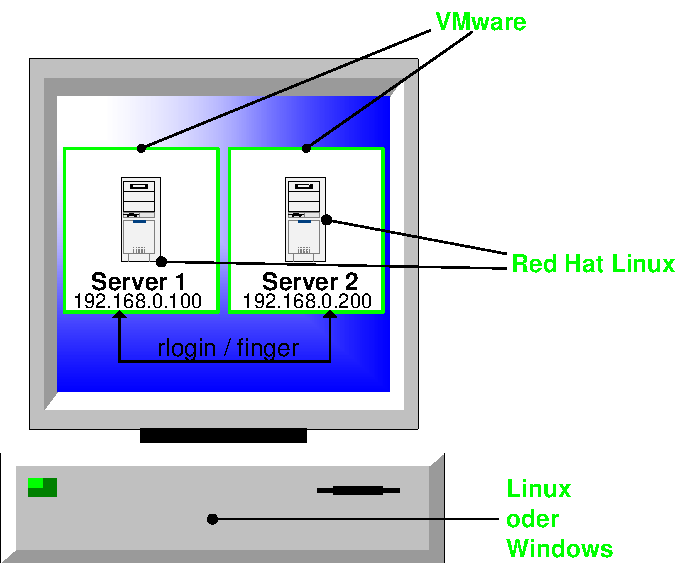
\includegraphics[width=10cm]{./files/inc/pictures/pdf/uebungsuebersicht}
		\caption{\label{pic:uebungsumgebung}�bungsumgebung}
	\end{center}
\end{figure}
\section*{Ausblick}
Mit dem H�rten kann ein Systems sehr sicher gemacht werden. Dennoch gibt es andere Techniken, welche die Sicherheit ebenfalls verbessern. Diese Techniken sind keine Konkurrenz zum H�rten, sondern viel mehr eine Erg�nzung. Um einen gesamthaften �berblick �ber die Thematik Sicherheit geben zu k�nnen, m�sste man diese Techniken ebenfalls ber�cksichtigen. Zudem umfasst das H�rten eines Systems mehr Punkte, als in diesem Dokument beschrieben wurden. Die Auswahl erfolgte nach der Wichtigkeit aus der Sicht der Autoren. Es ist denkbar, diese Punkte mit Fehlenden zu erg�nzen.
Die Ausf�hrliche Dokumentation der Recherchen f�r die �bung geeigneter Attacken zeigt, dass eine erfolgreiche Attacke, die dem Angreifer zu den Benutzerrechten eines Administrators verhilft nur mit sehr grossem Aufwand realisiert werden kann. Dies liegt vor allem daran, dass das Funnktionieren der Scripte von verschiedenen  Variablen der Systemkonfiguration des anzugreifenden Systems abh�ngen. Dazu geh�ren unter anderen die Version des Betriebssystems (oft auch die Version des Kernels) und die Version des anzugreifenden Dienstes. Darum ist es schwieriger f�r ein konkretes System einen funktionierenden Exploit zu finden, als mit einem Exploit-Script auf dem ganzen Internet ein angreifbares System.

Die entstandene �bung kann beliebig erweitert werden. Die in der erarbeiteten Form bereitgestellten Fragen k�nnen je nach Anwendung und Anforderung umformuliert bzw. erg�nzt werden.

\tableofcontents
%\listoffigures
%\listoftables

%%files einf�gen
\cleardoublepage
\pagenumbering{arabic}
\part{Einf�hrung}
\label{par:Einfuehrung}
\vspace{2cm}
Es werden grundlegende Begriffe erkl�rt und es wird ein Einblick in die Thematik Sicherheit gegeben.

	\chapter{Einleitung}
\label{cha:Einleitung}

Diese Arbeit besch�ftigt sich mit dem H�rten eines System. Im Internet und in der Literatur stolpert man oft �ber diesen Begriff, wenn �ber Sicherheit geschrieben wird. Da der Begriff und der Vorgang des H�rtens nicht im eigentlichen Sinne definiert sind, gibt es sehr unterschiedliche Meinungen dar�ber, was H�rten bedeutet und was es alles umfasst. Die vorliegende Arbeit soll einen Eindruck vermitteln, was unter H�rten eines Systems verstanden werden kann. Sie kann keine allgemeing�ltige Referenz sein, da je nach Einsatzgebiet eines Systems der Begriff unterschiedlich aufgefasst werden kann. Die Arbeit umfasst eine Zusammenstellung von Verfahren, die nach umfassendem Studium der Literatur den Autoren als wichtig erschienen. Welche davon im einzelnen Falle angewendet werden, h�ngt von der pers�nlichen Einstellung und der Verwendung ab. Da diese Arbeit nicht den Anspruch hat, jedes Gebiet der Sicherheit zu durchleuchten, beschr�nkt sie sich auf die folgenden Punkte:
\begin{itemize}
	\item	H�rten eines Systems 
	\item	Linux als Betriebs- und Serversystem
	\item	VMWare
\end{itemize}
und l�sst folgende Punkte aus:
\begin{itemize}
	\item	Intrusion Prevention und Produkte die dieses Prinzip implementieren (z.B. Stormwatch)
	\item	Secure Application Environment (basierend auf dem Produkt PitBull LX)
	\item	Intrusion Detection
	\item	Windows als Betriebssystem
	\item	PitBull
\end{itemize}

Im Zusammenhang mit H�rten treten in der Literatur verschiedene Begriffe auf, die z.T. verwirrend sein k�nnen. Im Englischen wird von "`System Hardening"'\index{System Hardening}, "`OS Hardening"'\index{OS Hardening} oder von "`Application Hardening"'\index{Application Hardening}  gesprochen. Mit dieser Unterteilung will man darauf hinweisen, dass es verschiedene Ebenen\index{H�rten!Ebenen} des H�rtens gibt. Diese sind in Tabelle \ref{tab:hardEbenen} zusammengefasst und erkl�rt. Wenn immer diese Unterteilung nicht von Bedeutung ist, wird der deutsche Begriff \emph{H�rten} bzw. \emph{H�rten eines Systems} f�r alle Ebenen verwendet. Die Definition, was darunter zu verstehen ist, wird in Kapitel \ref{sec:WasIstHaerten} gegeben.

\LTXtable{\linewidth}{./files/inc/tables/hardEbenen}

Weitere in diesem Dokument verwendeten Begriffe und Abk�rzungen sind in einem Glossar auf Seite \pageref{cha:Glossar} zusammengefasst.

Das Literaturverzeichnis mit s�mtlichen von uns verwendeten Referenzen befindet sich auf Seite \pageref{bibliography}.

Als Resultat der Arbeit ist eine �bung vorgesehen, die im Fach Internetsicherheit die M�glichkeit gibt, die hier erkl�rten Prinzipien und Verfahren selbst auszutesten, um sie besser zu verstehen.

Die Texte wurden bewusst nicht immer in rein \glqq technischer Sprache\grqq\ verfasst. Die Autoren hoffen, dass die Texte dadurch angenehmer und verst�ndlicher zu lesen ist.




	\chapter{Sicherheit}
\index{Sicherheit}
\label{cha:Sicherheit}

%----------
\section{Was ist Sicherheit}
\label{sec:WasIstSicherheit}
Sicherheit hat sehr viele Aspekte\index{Sicherheit!Aspekte}. Diese k�nnen grunds�tzlich in drei, f�r diese Arbeit relevanten, Hauptkategorien unterteilt werden:
\begin{itemize}
	\item	Schutz der Vertraulichkeit der Daten\index{Vertraulichkeit} (Data confidentiality)
	\item	Datenintegrit�t\index{Datenintegrit�t} (Data integrity)
	\item	Verf�gbarkeit des Systems\index{Verf�gbarkeit} (System availability)
	\end{itemize}
Der erste Punkt, Schutz der Daten, umfasst den Bereich der pers�nlichen Daten. Das System soll gew�hrleisten k�nnen, dass diese Daten geheim bleiben und nur den vom Besitzer festgelegten Personen zug�nglich sind. 

Unter Datenintegrit�t versteht man, dass Daten nur von berechtigten Benutzern ver�ndert werden k�nnen bzw. detektiert werden kann, von wem die �nderungen vorgenommen wurden. Ver�ndern heisst dabei auch l�schen oder hinzuf�gen von falschen Daten.

Die Verf�gbarkeit eines Systems ist ein sehr wichtiger Punkt im Bereich der Sicherheit. Es geht darum, dass niemand das System so st�ren kann, dass es unbenutzbar wird. Ein Stichwort hierbei ist \glqq denial of service\grqq \index{Denial of Service}. Personen die diese Attacken durchf�hren versuchen ein System so stark auszulasten, dass die bereitgestellten Dienste nicht mehr genutzt werden k�nnen.

Nat�rlich ist jedes einzelne der oben genannten Gebiete f�r sich sehr viel komplexer zu verstehen als hier angedeutet. Am technisch schwierigsten zu bek�mpfen sind die denial-of-service Attacken. F�r die beiden anderen Punkte gibt es bereits gute L�sungen.

Ein weiterer Aspekt, der immer zu heftigen Diskussionen f�hrt, ist die Privatsph�re\index{Privatsph�re}. Ein System soll die Person, die es benutzt, davor sch�tzen, dass private Informationen �ber die Person selbst f�r Dritte einsehbar sind. Das f�hrt schnell zu einer Diskussion �ber Moral bzw. zu der Frage nach der Legalit�t. Soll z.B. ein Staat ein Dossier �ber Computerbenutzer f�hren d�rfen, die sie zur Bek�mpfung von Internetkriminalit�t verwenden? Solche Themen sind sehr spannend, sollen aber nicht im Rahmen dieser Arbeit behandelt werden.

%----------
\section{Warum Sicherheit}
\label{sec:WarumSicherheit}
Die meisten Benutzer des Internets beachten das Gesetz. Das heisst sie versuchen nicht, andere zu sch�digen. Leider sind offensichtlich nicht alle Benutzer so. F�r sie gibt es einen englischen Begriff: \glqq intruders\grqq\ \index{intruder|see{Eindringlinge}}(Eindringlinge)\index{Eindringlinge} oder manchmal auch \glqq adversaries\grqq\ (Gegner). Diese Personen k�nnen grunds�tzlich in zwei Kategorien eingeteilt werden. Passive Eindringlinge\index{Eindringlinge!Passive} m�chten nur Daten lesen, f�r die sie keine Berechtigung haben. Aktive Eindringlinge\index{Eindringlinge!Aktive} m�chten diese Daten auch �ndern und sind somit eine gr�ssere Gefahr. Zudem kann noch zwischen Attacken die auf ein Ziel gerichtet sind (targeted) und Attacken die ein zuf�lliges Ziel aussuchen (opportunistic) unterschieden werden.

Nat�rlich gibt es nicht nur Personen, die Schaden anrichten, sondern noch andere Arten von Gefahren. Dies kann ein Wurm \index{W�rmer} (worms), ein Virus \index{Virus} oder ein Trojanisches Pferd \index{Trojanische Pferde} (trojan horse) sein. All das sind kleine Programme mit dem Ziel, Schaden auf einem Rechner anzurichten. Dabei ist es in den meisten F�llen f�r den Programmierer nicht entscheidend wo der Schaden entsteht. Es sind also zuf�llige Ziele. 

Die Kosten die durch Viren\index{Viren!Kosten} verursacht werden sind betr�chtlich. Sie werden f�r das Jahr 2000 auf \$$1.6*10^{12}$ gesch�tzt \footnote{Sch�tzung von PricewaterhouseCoopers, 2000}. 

Zus�tzliche Informationen und Berichte zu den Auswirkungen gibt es auf der Webseite von Securitystats \cite{secstats}. Einen Guten �berblick und eine Einf�hrung in das Thema Sicherheit bietet auch das Buch von Andrew. S. Tanenbaum \cite{Tanenbaum}.

%----------
\section{Wie sicher ist sicher?}
\label{sec:WieSicherIstSicher}
Eines muss schon zu Beginn klargestellt werden: Ein System ist und kann niemals vollkommen sicher sein. Es kann aber einem potenziellen Angreifer m�glichst schwierig gemacht werden, in das System einzudringen.

Ein weiterer Punkt den es zu beachten gilt ist, dass ein System zwar sehr sicher gemacht werden kann, unter Umst�nden dadurch aber die M�glichkeiten des Systems eingeschr�nkt werden. Zum Beispiel kann ein Server ohne Netzwerkverbindung laufen, dadurch wird er aber nahezu unbrauchbar. Somit ist es immer ein Balanceakt zwischen Sicherheit und Flexibilit�t bzw. Brauchbarkeit. Man sollte sich also immer �berlegen, f�r was das System eingesetzt werden soll. Weiter muss entschieden werden, wie wichtig die Daten sind, die zu sch�tzen sind bzw. wie gross der Schaden ist, falls die Daten verloren gehen oder gestohlen werden. Ebenso wichtig ist es zu entscheiden, wem man vertraut und Zugriff auf das System gew�hrt. Diese Entscheide bestimmen den Grad der Sicherheit nach denen ein Sicherheitsplan erstellt werden sollte.

%----------
\section{Was kann sicher gemacht werden?}
\label{sec:WasKannSicherGemachtWerden}
Technisch gesehen gibt es auf einem System verschiedene Stufen, auf denen das System sicherer Gemacht werden kann. Eine sehr ausf�hrliche Erkl�rung dazu kann im Linux Security-HOWTO \cite{secHowto} gefunden werden. Hier aber dennoch ein �berblick �ber die verschiedenen Stufen. Auf gewisse Punkte wird in dieser Arbeit in den folgenden Kapiteln genauer eingegangen.
\begin{itemize}
	\item	Physical Security (physikalische Sicherheit)
	\item	Local Securtiy (lokale Sicherheit)
	\item	Files and File system Securtiy (Datei- und Dateisysteme sch�tzen)
	\item	Password Securtiy and Encryption (Passw�rter und Verschl�sselung)
	\item	Kernel Securtiy
	\item	Network Security (Netzwerksicherheit)
\end{itemize}
Dies ist eine technische Unterteilung. Auf Bereiche wie \glqq Social Engineering\grqq \index{Social Engineering} oder \glqq Security Awareness\grqq \index{Security Awareness} wird hier nicht eingegangen.

%----------
\section{Probleme}
\label{sec:Probleme}
Das Hauptproblem im Bereich der Sicherheit ist, wie oben schon angesprochen, dass ein System niemals sicher sein kann. Der Grund sind fehlerhafte Applikationen. Dass Applikationen Fehler aufweisen l�sst sich aus verschiedenen Gr�nden nicht vermeiden, z.T. wegen des Zeitdruckes (\glqq time-to-market\grqq) oder auch wegen der wachsenden Komplexit�t der Programme. Das Einzige was dagegen gemacht werden kann, ist, sobald ein Fehler entdeckt wurde, ihn zu beheben und sofort einen Patch f�r die Kunden bzw. Benutzer des Programms bereitzustellen. Der Nachteil darin ist, dass der Patch erst gemacht werden kann, wenn das Sicherheitsproblem erkannt wurde (oft durch eine Attacke). Das gleiche gilt f�r Applikationen, die das System sch�tzen sollen (z.B. ein Virenschutz). Diese Applikationen sch�tzen das System nur vor bekannten Angriffen. Diese Systeme werden reagierende System (reactive Systems)\index{reagierende Systeme} genannt. Das heisst, sie k�nnen nur reagieren, was bedeutet, dass der Angreifer bereits in das System eingedrungen ist. Es gibt aber auch einen Ansatz der versucht, Attacken zu erkennen, bevor jemand ins System eindringen kann. Diese werden agierende System (proactive Systems) (Agierende Systeme)\index{agierende Systeme} genannt. Sie versuchen gewisse Muster, die auf eine Attacke hinweisen, zu erkennen. Wie immer ist agieren die bessere L�sung als reagieren, aber sehr viel schwieriger zu realisieren.

In den folgenden Kapiteln werden verschiedene Ans�tze zur Verhinderung von Attacken aufgezeigt und genauer erkl�ren.



	
\part{Sicherheitstechnologien}
\label{par:Sicherheitstechnologien}
\vspace{2cm}
Es werden verschiedene Technologien vorgestellt, die zur Sicherheit eines Systems beitragen k�nnen, bzw. f�r die �bung verwendet werden. Genauer betrachtet wird in diesem Teil die Technik des H�rtens und PAM (Pluggable Authentication Module).
Im Softwareteil befindet sich eine kurze Erl�uterung der Funktionalit�t von PitBull, der Kommandos \verb~rlogin~, \verb~finger~, \verb~arp~ und eine Beschreibung der Konfiguration von VMware.
	\chapter{H�rten eines Systems \index{H�rten|(}}
\label{cha:HaertenEinesSystems}
Es ist die Aufgabe eines Administrators eines Systems, dieses so sicher wie m�glich oder so sicher wie n�tig zu machen. Um die Sicherheit zu erh�hen gibt es verschiedene, nahezu unendlich viele M�glichkeiten. Aus diesem Grund ist es schwierig, eine "`Anleitung"' zu schreiben. Es kann hier lediglich eine Auswahl von M�glichkeiten gegeben werden, die helfen k�nnen, die Sicherheit zu erh�hen. Es soll einen �berblick geben und soll gleichzeitig ein Gef�hl daf�r geben, was alles beachtet werden sollte. 

%----------
\section{Was ist H�rten eines Systems?}
\label{sec:WasIstHaerten}
Eine Definition \index{H�rten!Definition} von \glqq H�rten eines Systems\grqq\ ist wie folgt:
\begin{quote}
``System hardening is a step by step process of securely configuring a system to protect it against unauthorized access, while also taking steps to make the system more reliable. Generally anything that is done in the name of system hardening ensures the system is both secure and reliable.''\footnote{Definition von \url{http://www.itcoach.com/unsafe/System-Hardening.htm}}
\end{quote}

H�rten eines Systems bedeutet damit, ein System so zu konfigurieren, dass es sicher und zuverl�ssig ist. Dies umfasst nicht nur, bekannte Sicherheitsprobleme zu l�sen bzw. zu umgehen, sondern es umfasst auch die Frage, welche Services auf dem System laufen m�ssen.

Oft wird eine Unterteilung\index{H�rten!Unterteilung} gem�ss Tabelle \ref{tab:securitylevels} gemacht. In dieser Arbeit wird diese Unterteilung nicht gemacht, da es oft schwierig ist, einzelne Punkte in eine Kategorie einzuteilen. Ausserdem ist es nicht entscheidend, in welche Kategorie diese Punkte fallen, wichtig ist nur, dass sie Sicherheitsrelevant sind und deshalb auch beachtet werden. Aus diesem Grund ist der Prozess des H�rtens nicht in Kategorien unterteilt, sondern wird anhand eines Ablaufes dargestellt, der alle Kategorien enth�lt.

\LTXtable{\linewidth}{./files/inc/tables/securitylevels}

%----------
\section{Prinzipien des H�rtens}\index{H�rten!Varianten}
\label{sec:HardeningPrinzipien}

Es gibt verschiedene Ans�tze, ein System zu H�rten. Zum einen k�nnen alle Einstellungen manuell gemacht werden. Das heisst, die Konfigurationen der Programme, die auf dem System laufen, werden von Hand angepasst um deren Sicherheit zu erh�hen. Eine weitere M�glichkeit ist, Linux-Tools zu Hilfe zu nehmen. Diese versuchen die Konfiguration der Programme nach den Aspekten der Sicherheit vorzunehmen. Die dritte M�glichkeit ist schliesslich, ein Produkt einzusetzen, welches das Prinzip des H�rtens implementiert. Die zwei letzten Varianten unterscheiden sich grunds�tzlich nicht durch die Art und Weise, wie sie das Problem angehen. Meist unterst�tzen aber kommerzielle Produkte nicht nur das H�rten, sondern haben noch andere sicherheitsrelevanten Teile implementiert. Die verschiedenen Varianten sind in Tabelle \ref{tab:hardprinc} zusammengefasst:
\pagebreak

\LTXtable{\linewidth}{./files/inc/tables/hardprinc}


%----------
\section{Manuelles H�rten \index{H�rten!manuell}}
\label{sec:ManuellesHaerten}
Bei der manuellen Konfiguration der Programme, kann das System sehr spezifisch eingerichtet werden. Das ist ein grosser Vorteil gegen�ber der automatischen Anpassung der Konfigurationen, bedeutet aber auch, dass der Systemadministrator mehr Wissen �ber die auf dem Server eingesetzte Software haben muss. Grunds�tzlich sollte man sich dabei folgende Punkte �berlegen:
\begin{itemize}
	\item	Welche Dienste werden auf dem System wirklich ben�tigt?
	\item	Welcher Benutzer hat welche Berechtigungen auf dem System?
	\item	Wie ist das System zu H�rten, damit bei einer Kompromittierung nicht das ganze System betroffen ist?
	\item	Welche Programme sind geeignet, um unberechtigte Zugriffe zu erkennen und aufzeichnen zu k�nnen?
\end{itemize}
Diese Punkte sind entscheidend und gelten nicht nur f�r die manuelle Konfiguration, sondern f�r alle Vorgehensweisen. Am meisten Gedanken wird man sich aber bei der manuellen Konfiguration machen m�ssen. In der vorliegenden Arbeit geht es nicht um das Erkennen von unberechtigten Zugriffen, trotzdem sollte man wissen, dass es auch zum H�rten eines Systems geh�rt.

\subsection{Ablauf vor und w�hrend der Installation}
Folgendes ist ein Vorschlag, ein System zu H�rten. Die Liste ist nicht abschliessend, sie soll viel mehr einen �berblick geben, worum es in dem Prozess geht und dabei soll verst�ndlich gemacht werden, was H�rten eines Systems bedeutet. 

\begin{enumerate}
	\item	W�hlen Sie ein BIOS Passwort\index{BIOS Passwort} und stellen Sie sicher, dass das System nur von der Festplatte gestartet werden kann (booten mit Diskette, etc. abstellen). Damit verhindern Sie, dass jemand, der physischen Zugriff zum Rechner hat, diesen mit einer Diskette oder CD Rom booten kann.
	\item	W�hlen Sie ein geeignetes Dateisystem\index{Dateisystem w�hlen} und partitionieren\index{Partitionierung} Sie die Festplatte. Was eine sinnvolle Partitionierung bedeutet h�ngt vom Einsatz des Systems ab. Zum Beispiel sollte ein System, das als Mailserver eingesetzt wird, eine eigene Partition f�r den Mail Spooler\footnote{Ein Mail Spooler ist f�r die Versendung und das Verteilen von Mails zust�ndig} haben (\verb~/var/mail~ und/oder \verb~/var/mail/spool~). Damit wird verhindert, dass  ein Benutzer den Mail Spool und damit die ganze Festplatte f�llen kann. Folgende Punkte sind Vorschl�ge, die beachtet werden sollten.
	\begin{itemize}
		\item	Es sollten sich alle Verzeichnisse, auf die ein Benutzer Schreibrecht hat, auf einer eigenen Partition befinden. Dies umfasst zum Beispiel \verb~/home~ und \verb~/tmp~. Das reduziert das Risiko einer "`user DoS"'\footnote{Das Bedeutet, ein Benutzer k�nnte die root Partition (\verb~/~) mit Daten auff�llen und damit das System unbenutzbar machen.} Attacke.
		\item	Partitionen die dynamisch ihren Inhalt �ndern, wie z.B. \verb~/var~ sollten ebenfalls auf eine eigene Partition, da sie sonst in kurzer Zeit �berf�llt werden k�nnten.
		\item	Partitionen, auf denen Software installiert wird, die nicht zur Distribution geh�rt, sollten auf einer eigenen Partitionen sein. Damit wird die Software bei einer allf�lligen Neuinstallation nicht gel�scht. Das hat nicht direkt mit dem H�rten eines Systems zu tun, hilft aber im Falle einer Neuinstallation.
		\item	Daten, die statisch sind, sollten auf einer eigenen Partition sein. Diese kann dann read-only gemountet werden.
	\end{itemize}
	
	Das gew�hlte Dateisystem kann im Fall eines Absturzes Auswirkungen haben. Das Standarddateisystem ist \verb~ext2~. Es wird aber empfohlen, ein journalling Dateisystem wie z.B. \verb~ext3~ zu w�hlen. Die Wahrscheinlichkeit Daten zu verlieren ist damit kleiner (zudem ist \verb~ext3~ im Betrieb schneller).
	\item	W�hlen Sie ein sicheres root Passwort\footnote{\label{fn1}ein sicheres Passwort ist mind. 6 Zeichen lang, hat mind. 2 alphabetische Zeichen und 1 numerisches oder 1 spezial Zeichen. Das Passwort muss vom user login verschieden sein und darf auch nicht davon abgeleitet werden k�nnen. Es darf zudem nicht von einem Wort oder einer Wortkombination abgeleitet werden k�nnen.}\index{Passw�rter}. Das ist ein grundlegender Schritt um ein sicheres System zu bekommen. Am Besten verwenden Sie dazu einen Passwortgenerator. Diese generieren je nach Programm sehr sichere Passw�rter (z.B. \textit{makepasswd}\index{makepasswd@\texttt{makepasswd}} unter Linux).
	\item	Schalten sie "`Shadow Password"'\index{Shadow Passwort} ein. Shadow Password bedeutet, das Passwort wird in \verb~/etc/shadow~ gespeichert und kann nur noch vom user \verb~root~ und von der Gruppe \verb~shadow~ gelesen werden. Damit wird verhindert, dass ein Angreifer eine Kopie der Passwortdatei bekommen kann und einen Passwort Cracker darauf ansetzt.
	\item	Finden Sie heraus, welche Dienste auf dem System laufen. Installieren und starten Sie nur die ben�tigten Dienste. Dienste sind Programme wie z.B. ein ftp-Server (z.B. \textit{Proftp}) oder ein Webserver (\textit{Apache}). �berlegen Sie sich, was sie auf Ihrem System wirklich anbieten wollen und schalten Sie alle anderen Dienste aus. Der Grund liegt darin, dass Netzwerkdienste auf eine Verbindung von ausserhalb warten. Diese Dienste k�nnen (auch unbekannte) Sicherheitsl�cken aufweisen und sind damit eine Gefahr. Stellen Sie weiter sicher, dass beim Aufstarten kein Dienst, den sie nicht brauchen, versucht wird vom Betriebssystem zu starten.
	\item	�berpr�fen  und berichtigen Sie die Zugriffsberechtigungen\index{Zugriffsberechtigungen} auf die Dienste. Es sollen nur Benutzer Zugriff auf einen Dienst erhalten, die ihn wirklich ben�tigen. Oft ist das nur der user root.
	\item	Installieren Sie nur die Pakete bzw. Programme, die Sie wirklich auf Ihrem System ben�tigen. Jede �bliche Linux Distribution (z.B. SuSE, RedHat, Debian, etc.) beinhaltet tausende von Programmen. W�hlen Sie aus denen nur die ben�tigten aus, damit Sie nicht Programme installiert haben, die es einem Angreifer erleichtern k�nnen eine Attacke durchzuf�hren. Erleichtert wird die Auswahl bei den meisten Distributionen dadurch, dass die Programme in Kategorien unterteilt sind, die nach Bedarf komplett ausgeschaltet werden k�nnen. Achten Sie bei der Auswahl der Programme darauf, dass Sie als sicher geltende Programme installieren. 
	\item	Updaten aller installierten Pakete, um jedes Paket auf den aktuellsten Stand zu setzen.
	\item	Gew�nschte "`user accounts"' anlegen. Dabei soll beachtet werden, dass sichere Passw�rter verwendet werden. Dabei gelten die gleichen Regeln wie beim Anlegen eines root Passwortes.
\end{enumerate}

\subsection{Ablauf nach der Installation}
Wenn die im letzten Abschnitt beschriebenen Schritte durchgef�hrt sind, ist das System installiert und lauff�hig. Trotzdem kann noch mehr getan werden, um das System sicher zu machen. Dies ist wieder eine Auswahl, die nicht abschliessend ist.
\begin{enumerate}
	\item	Setzen Sie ein Bootmanager\index{Bootmanager Passwort} (\textit{Lilo} oder \textit{Grub}) Passwort. Haben Sie kein Bootmanager Passwort, kann jemand, der root Berechtigung auf dem System erlangt hat, das root Passwort �ndern und das System neu starten. In diesem Fall haben Sie keinen Zugriff mehr auf Ihr System, da sie das Passwort nicht mehr kennen. Die einzige L�sung ist dann eine komplette Neuinstallation. Mit einem Bootmanager Passwort verhindern Sie den Neustart ohne Passwort. Das gew�hlte Passwort sollte nat�rlich verschieden vom root Passwort sein.
	\item	Schr�nken Sie den Zugriff auf das System �ber das Netz ein. Das bedeutet, ein Benutzer muss sich zuerst mit einen Benutzernamen/Passwort einloggen, um dann mit \verb~su~ oder \verb~sudo~ root Rechte zu bekommen. Damit wird verhindert, dass sich jemand direkt als root einloggen kann und hat zudem den Vorteil, dass ein direkter Angriff auf das root Passwort sinnlos wird, da zuerst ein Benutzerpasswort gefunden werden muss.
	\item Falls Personen physischen Zugriff zum System haben, erlauben Sie nur bestimmten Personen, beim System einen Neustart durchzuf�hren. Wenn Sie die Standardeinstellung beibehalten kann \emph{jeder} das System neu starten (mit der Tastenkombination \verb~Ctrl-Alt-Del~).
	\item Achten Sie beim mounten\index{Mounten} von Partitionen darauf, dass Sie auf bestimmten Partitionen keine Ausf�hrung von Programmen erlauben (z.B. auf der Partition \verb~/tmp~). �berpr�fen Sie die Mountingtabelle (\verb~/etc/fstab~) und setzen Sie die Optionen entsprechend\footnote{Details zu den Optionen erhalten Sie in der Manual Page des mount Befehls (\verb~man mount~)}.
	\item Informieren Sie sich �ber Sicherheitsupdates die Ihre Software betrifft. Am besten in einer Security Announce Mailing List.
	\item Mit PAM\index{PAM} (Pluggable Authentication Module) k�nnen Sie festlegen, wie Benutzer von den Programmen authentifiziert werden. Das heisst, der Zugriff auf Programme kann geregelt werden. Da die Authentifizierung ein sehr zentraler Punkt ist, ist dieser ein eigener Abschnitt gewidmet. Siehe \ref{sec:Authentifizierung}. 
	\item Limitieren Sie die Resourcen\index{PAM!Resourcen zuteilen}, die ein Benutzer belegen kann. Ohne diese Massnahme kann \emph{jeder} Benutzer so viel CPU Rechenleistung und Speicher belegen wie er will. Dies bedeutet, jeder kann das System auslasten bzw. �berlasten. Sie k�nnen mit PAM (s. oben) einstellen, wieviel Rechenleistung, Speicher, etc., Sie jedem Benutzer zuteilen wollen. Genau genommen k�nnen mit PAM alle Resourcen des Systems eingeteilt werden. Damit ein Benutzer nur einen Teil des Festplattenspeichers belegen kann, k�nnen Sie pro Benutzer eine quota anlegen. Detaillierte Informationen dazu k�nnen unter \url{http://seifried.org/lasg/users/} gefunden werden.
	\item Wenn sich ein Benutzer mit einem falschen Benutzernamen und/oder Passwort einloggt, muss er eine kurze Zeit warten, um einen neuen login promt zu erhalten. Erh�hen Sie diese Zeit dynamisch, das heisst, bei jedem Fehlversuch wird die Zeit erh�ht. Damit erschweren Sie einem potentiellen Angreifer einen "`Brute Force"'\footnote{Dabei werden alle m�glichen Paare von Benutzername/Passwort systematisch durchprobiert bis ein g�ltiges Paar gefunden wurde} Angriff auf das System, da es sehr zeitaufw�ndig wird. Sie k�nnen den Benutzer auch nach 3 Fehlversuchen sperren. Sie sollten die Login-Versuche in einer Logdatei festhalten.
	\item Falls es n�tig ist, dass Benutzer auf dem System root Rechte bekommen, sollten Sie statt dem Befehl \verb~su~\index{su@\texttt{su}} den Befehl \verb~sudo~\index{sudo@\texttt{sudo}} verwenden. Dieser bietet mehr M�glichkeiten, z.B. kann in der Konfigurationsdatei bestimmt werden, welche Befehle von welchem Benutzer ausgef�hrt werden d�rfen. Zus�tzlich gibt es bei der Eingabe eines falschen Passwortes einen Eintrag in der Logdatei und diese wird dem Administrator als Mail zugesandt.
	\item Limitieren Sie die Rechte des Benutzers und zeichnen Sie dessen Aktivit�ten auf. Zum Beispiel sollten die Rechte der Dateien\index{Dateirechte} angepasst werden, damit der Benutzer nur die Dateien lesen kann, die n�tig sind. Es k�nnen auch die Standardvorgaben f�r das Erstellen von Dateien ge�ndert werden, damit diese nur noch vom Benutzer selbst lesbar sind (\verb~umask~). Im Bereich der Aufzeichnungen gibt es viele M�glichkeiten, angefangen vom Aufzeichnen des Anmeldens bis hin zum Aufzeichnen jedes einzelnen Zeichens, das der Benutzer eingibt. Hier ist ein sinnvolles Mittelmass zu finden (\textit{syslog}).
	\item �berpr�fen Sie die Passw�rter, die von den Benutzern gew�hlt wurden, oder noch besser, lassen Sie nur sichere Passw�rter zu, in dem Sie bereits beim Erstellen Wortlisten verwenden und dem Benutzer nur erlauben, Passw�rter zu benutzen, die mit keinem Wort in den Wortlisten in Verbindung gebracht werden k�nnen. Am Besten verwenden Sie f�r die �berpr�fung \textit{cracklib}\index{cracklib} mit einer der Wortliste \textit{cracklib\_dict}. F�r die Passw�rter gelten die Anforderungen, die in der Fussnote \ref{fn1} beschrieben sind.
	
	Um nachtr�glich zu �berpr�fen ob die gew�hlten Passw�rter sicher sind, gehen sie genauso vor wie ein Angreifer. Verwenden Sie einen Passwort cracker\index{Passwort Cracker} wie z.B. \textit{john}\index{johntheripper}\footnote{Dieses Programm kann von \url{http://www.openwall.com/john/} heruntergeladen werden.} zusammen mit Wortlisten. Wenn Sie ein Passwort knacken k�nnen, haben Sie eine Sicherheitsl�cke entdeckt und k�nnen entsprechende Massnahmen ergreifen.
	\item Es ist wichtig zu entscheiden, wer Zugriff zu den Logdateien hat, da diese oft sehr genaue Informationen �ber ein System liefern. Zudem werden sie nutzlos, wenn ein Angreifer die Logdateien nach einem erfolgreichen Angriff �ndern kann.
	\item Sie k�nnen Ihr System sicherheitstechnisch in vielen Hinsichten verbessern, wenn Sie den Kernel optimieren. Viele Distributionen bieten "`Kernel Patches"' an, die die Sicherheit verbessern. Viele �nderungen k�nnen zur Laufzeit angepasst und ver�ndert werden. Dazu dient der Befehl \verb~sysctl~\index{sysctl@\texttt{sysctl}}. Er erlaubt zum Beispiel das Ignorieren von icmp requests, aber nat�rlich noch vieles mehr. Informationen dazu finden Sie ebenfalls in der Manpage (\verb~man sysctl~).
	\item Sobald Ihr System fertig konfiguriert ist, machen Sie ein Snapshot von dem System. Dies beinhaltet ein \verb~md5sum~ der wichtigsten Verzeichnisse (z.B. boot). Damit k�nnen Sie jederzeit �berpr�fen, ob ihr System noch im originalen Zustand ist.
\end{enumerate}


Das ist der Ablauf, um ein System zu H�rten. Die konkreten Einstellungen die gemacht werden m�ssen, sind in diesem Ablauf nicht beschrieben, da sie Distributionsabh�ngig sind. F�r Debian k�nnen die Einstellungen im Securing Debian Manual \cite{secDebian} nachgelesen werden. F�r andere Distributionen gibt es jeweils sehr umfangreiche Dokumentationen, die auf den Webseiten gefunden werden k�nnen.

\subsubsection{Beispiel ssh}\index{H�rten!Beispiel ssh}\index{ssh h�rten}
Da im obigen Ablauf nur die Schritte, nicht aber die konkreten Einstellungen zum H�rten eines Systems beschrieben wurden, soll hier stellvertretend f�r andere Dienste der \textit{ssh} Dienst genauer betrachtet werden.

Falls Sie anstatt \textit{ssh} immer noch \textit{telnet} verwenden, sollten Sie \textit{telnet} abschalten und stattdessen als externe Zugriffsm�glichkeit nur noch \textit{ssh} verwenden. Anschliessend sollten Sie folgende Einstellungen in der \textit{OpenSSH} Konfigurationsdatei machen:
\begin{itemize}
	\item	\verb~ListenAddress IPx~\\ \textit{ssh} soll nur auf einem \glqq Interface\grqq\ auf Verbindungen warten. Diese Einstellung ist n�tig, falls Sie mehrere Netzwerkkarten haben, damit Sie die Zugriffe besser kontrollieren k�nnen. Ausserdem k�nnen Sie den Zugriff einschr�nken, indem Sie z.B. den Zugriff nur von innerhalb Ihres Netzes zulassen, von Ausserhalb jedoch sperren.
	\item	\verb~PermitRootLogin No~ \\Es darf sich niemand direkt als root einloggen. Will jemand root Rechte via \textit{ssh} bekommen, ist zweimaliges Einloggen erforderlich. Das heisst ein "`Brute Force"' Angriff auf das root Passwort wird sinnlos, da auch ein g�ltiges root Passwort nicht akzeptiert wird.
	\item	\verb~Listen Port xy~\\ �ndern Sie den port (Standardport f�r \textit{ssh} ist Port 22), auf den \textit{ssh} auf Verbindungen wartet. Damit kann niemand ganz sicher sein, ob der \textit{ssh} Dienst wirklich l�uft. \emph{Wichtig:} Diese Option ist \glqq security by obscurity\grqq\ (Sicherheit durch Verwirrung) und dient dazu, unerfahrene Angreifer zu verwirren.
	\item	\verb~PermitEmptyPasswords no~\\Leere Passw�rter d�rfen niemals erlaubt werden.
	\item	\verb~AllowUsers name ref user@host~\\ Es wird nur bestimmten Benutzern erlaubt, sich via \textit{ssh} einzuloggen. 
	\item	\verb~AllowGroups wheel admin~\\ Nur Mitglieder der angegebenen Gruppen (in diesem Beispiel die Gruppe \verb~wheel~ und \verb~admin~) d�rfen sich via \textit{ssh} einloggen.
	\item	\verb~PasswordAuthentication yes~\\Benutzer d�rfen sich mit einem Passwort anmelden. Die bessere L�sung ist, die Option auf \verb~no~ zu setzen, um nur den Zugriff via einem ssh-key zuzulassen. Ein Login via ssh-key basiert auf dem Prinzip der asymmetrischen Verschl�sselung. Das heisst, der Benutzer hat einen "`private key"' den sonst niemand kennt. Dieser wird zur Authentifizierung benutzt und kann damit nicht durch einen "`Brute Force"' Angriff herausgefunden werden, was grunds�tzlich bei einer Authentifizierung mit einem Passwort m�glich ist.
	\item	\verb~Protocol 2~\\Es soll nur die Protokoll Version 2 erlaubt sein. Version 1 hat einige Sicherheitsl�cken.
\end{itemize}

%----------
\section{Automatisches H�rten}\index{H�rten!automatisch}
\label{sec:automatischesHaerten}
Im vorangegangenen Abschnitt wurde beschrieben, wie ein System von Hand geh�rtet werden kann. Das sieht nach sehr viel Arbeit aus und tats�chlich ist es das auch. Man k�nnte sich die Frage stellen, ob es nicht ein Programm gibt, das einem die ganzen Einstellungsarbeiten abnimmt und den Vorgang des H�rtens automatisiert. Tats�chlich gibt es verschiedene Ans�tze, die genau das versuchen. Trotzdem muss gesagt werden, dass ein Programm nicht die ganze Arbeit ausf�hren kann. Sicherheit ist ein Prozess, der nicht bei der Konfiguration aufh�rt. Es gibt dauernd neue Programme, neue Angriffe, neue Gefahren. Ein Programm, dass ein System automatisch h�rtet, kann diesen Anforderungen nur in einem gewissen Masse nachkommen. Das bedeutet, auch beim Einsatz solcher Tools muss der Administrator seinen Teil leisten und muss mit dem System und mit den Gefahren vertraut sein. Es ist ein Irrtum, jeder k�nne mit dem geeigneten Programm ein sicheres System haben.

Im Folgenden werden zwei Produkte vorgestellt, die das H�rten automatisieren. Das eine ist das Paket \textit{harden}, das andere ist \textit{Bastille Linux}.

\subsection{Harden}\index{H�rten!automatisch!Harden}\index{Harden Programm}
Dieses Paket versucht es dem Administrator zu erleichtern, ein System zu installieren, das sicher und leichter zu administrieren ist. Es bringt eine schnelle Hilfe bei der Installation. Es deinstalliert Pakete mit bekannten Sicherheitsproblemen oder, soweit als m�glich, auch Programme, die Klartext �ber ein Netz �bermitteln, etc. Es installiert auch Tools, die die Sicherheit des Systems erh�hen sollen (Intrusion Detection Tools, Analysetools, etc.). Konkret wird folgendes installiert:
\begin{itemize}
	\item \verb~harden-doc~ \\Dokumentationen
	\item \verb~harden-tools~ \\Tools um die Sicherheit des Systems zu erh�hen, wie z.B. kernel patches, intrusion detection, etc.
	\item \verb~harden-environment~ \\Hilft eine Umgebung zu konfigurieren.
	\item \verb~harden-servers~ \\Entfernt Server, die als nicht sicher gelten (z.B. \textit{telnetd}).
	\item \verb~harden-clients~ \\Entfernt Clients, die als nicht sicher gelten (z.B. \textit{telnet}).
	\item \verb~harden-remoteflaws~ \\Entfernt Programme mit Sicherheitsl�cken, die es einem entfernten Angreifer erlauben, das System zu kompromittieren (Welche Programme das sind, h�ngt von den Programmen und deren Versionen ab).
	\item \verb~harden-localflaws~ \\Entfernt Programme mit Sicherheitsl�cken die es einem lokalen Angreifer erlauben, das System zu kompromittieren (Welche Programme das sind, h�ngt von den Programmen und deren Versionen ab).
	\item \verb~harden-remoteaudit~ \\Tools um ein System von einem entfernten Rechner aus zu �berwachen.
\end{itemize}
Das \textit{harden} Paket wird st�ndig erweitert und es ist deshalb m�glich, dass diese Aufz�hlung nicht mehr aktuell ist. Die aktuelle Version kann von \url{http://ftp.debian.org/debian/pool/main/h/harden/} heruntergeladen werden.

\subsection{Bastille Linux}\index{H�rten!automatisch!Bastille Linux}\index{Bastille Linux}
\textit{Bastille Linux} ist ein Tool, das ein  System automatisch h�rtet. Urspr�nglich wurde es f�r \textit{Red Hat} und \textit{Mandrake} entwickelt, funktioniert mittlerweilen aber auch f�r andere Distributionen. Bei \textit{Bastille Linux} gibt es verschiedene Modi, aus denen einer gew�hlt werden kann:
\begin{itemize}
	\item \textit{Bastille Linux} versucht anhand von Antworten zu Sicherheitsfragen das System zu konfigurieren. Diese Variante nennt sich \textit{InteractiveBastille}.
	\item Sicherheitsstufen (locker, moderat, paranoid) k�nnen gew�hlt werden. Je nach der gew�nschten Stufe wird das System konfiguriert. Diese Variante nennt sich \textit{BastilleChooser}
	\item Es wird eine bereits definierte Konfigurationsdatei genommen (z.B. von \textit{Bastille Linux}). Anhand dieser Datei wird ein Sicherheitskonzept auf dem System implementiert. Diese Variante nennt sich \textit{AutomatedBastille}.
\end{itemize}
Weitere Informationen zu diesem Projekt k�nnen auf \url{http://www.bastille-linux.org} gefunden werden.
\index{H�rten|)}

%----------
\section{Authentifizierung}\index{Authentifizierung}
\label{sec:Authentifizierung}

Ein wichter Aspekt der Sicherheit ist die Authentifizierung der Benutzer durch das System. Immer, wenn sich ein Benutzer einloggt, wird �berpr�ft, ob er Zugriff zum System hat und welche Rechte ihm gegeben werden sollen. In den Anf�ngen des Computerzeitalters hat es gereicht, einen Benutzer anhand des Namens und eines Passwortes zu identifizieren. Man glaubte jedem, der ein korrektes Passwort eingegeben hat, dass er auch wirklich derjenige Benutzer sei. Seit dem die Computer mehr und mehr vernetz wurden, kam der Anspruch dazu, dass man kontrollieren kann, woher sich ein Benutzer einloggt und was er auf dem System machen darf. Daraus sind komplexere Authentifizierungsmechanismen entstanden, die im Folgenden erkl�rt werden. Dies soll helfen zu verstehen, was genau passiert, wenn man sich auf einem System �ber ein Netzwerk oder lokal einloggt.

\subsection{Prozesse}\index{Prozesse unter Linux}
Um verstehen zu k�nnen, was bei einem login passiert wird hier ein kleiner �berblick der Prozesse unter Linux gegeben. Beim Starten des Systems wird zuerst der Kernel in den Hauptspeicher geladen. Dieser l�dt die Treiber f�r die Hardware und initialisiert sie. Anschliessend wird die root Partition (\verb~/~) gemountet und der erste Prozess gestartet. Dies ist der \emph{init} Prozess\index{init Prozess}\index{Prozesse unter Linux!init}. Dieser ist der Vater aller Prozesse. Von ihm werden alle anderen Prozesse abgeleitet. Dies kann man gut nachvollziehen, wenn man den Befehl \verb~pstree~\index{pstree@\texttt{pstree}} in der Konsole eingibt. Eine m�gliche Ausgabe k�nnte folgendermassen aussehen:
\begin{verbatim}
se@mandy: pstree -u
init-+-6*[agetty]
     |-bdflush
     |-cron
     |-devfsd
     |-dhcpcd
     |-eth0
     |-kapmd
     |-keventd
     |-klogd
     |-kreiserfsd
     |-ksoftirqd_CPU0
     |-kswapd
     |-kupdated
     |-lockd
     |-master-+-pickup
     |        `-qmgr
     |-portmap
     |-rpciod
     |-sshd---sshd---sshd---bash(se)---pstree
     `-syslogd
\end{verbatim}
Alternativ k�nnen die Prozesse und deren Hirarchie auch mit dem \verb~ps~\index{ps@\texttt{ps}} Befehl angeschaut werden. Dann sieht die Ausgabe bei gleichen Prozessen folgendermassen aus:
\begin{verbatim}
se@mandy: ps ax -H -o user,pid,tty,stat,command
USER       PID TT       STAT COMMAND
root         1 ?        S    init [3]
root         2 ?        SW     [keventd]
root         3 ?        SW     [kapmd]
root         4 ?        SWN    [ksoftirqd_CPU0]
root         5 ?        SW     [kswapd]
root         6 ?        SW     [bdflush]
root         7 ?        SW     [kupdated]
root         8 ?        SW     [kreiserfsd]
root        26 ?        S      /sbin/devfsd /dev
root       858 ?        SW     [eth0]
root       860 ?        S      /sbin/dhcpcd -t 30 -h mandy eth0
bin        930 ?        S      /sbin/portmap
root       934 ?        SW     [rpciod]
root       935 ?        SW     [lockd]
root      1014 ?        S      /usr/lib/postfix/master
postfix   1038 ?        S        pickup -l -t fifo -u
postfix   1039 ?        S        qmgr -l -t fifo -u
root      1051 ?        S      /usr/sbin/sshd
root      1134 ?        S        /usr/sbin/sshd
se        1136 ?        S          /usr/sbin/sshd
se        1137 pts/0    S            -bash
root      1110 ?        S      /usr/sbin/syslogd -m 0
root      1113 ?        S      /usr/sbin/klogd -c 3 -2
root      1116 ?        S      /usr/sbin/cron
root      1128 tty1     S      /sbin/agetty 38400 tty1 linux
root      1129 tty2     S      /sbin/agetty 38400 tty2 linux
root      1130 tty3     S      /sbin/agetty 38400 tty3 linux
root      1131 tty4     S      /sbin/agetty 38400 tty4 linux
root      1132 tty5     S      /sbin/agetty 38400 tty5 linux
root      1133 tty6     S      /sbin/agetty 38400 tty6 linux
\end{verbatim}
Wie man sieht, werden beim Start verschiedene Prozesse gestartet. Welche das sind, h�ngt von der Konfiguration und der Verwendung des Systems ab. Zum Beispiel wird hier noch der ssh Deamon (\textit{sshd}) gestartet. Was aber immer vom System bereit gestellt wird, sind mehrere tty\index{tty}. Ein tty ist ein virtuelles Terminal auf dem man sich einloggen kann. Der Begriff tty (TeleTYpe) stammt aus den Anf�ngen der Computergeschichte, als Computer noch riesige Anlagen im Keller waren und man sich mittels eines Terminals (meist nur ein Bildschirm, eine Tastatur und eine serielle Schnittstelle zum Computer) einloggen musste. Heute geschieht dies lokal, das Prinzip ist aber dasselbe geblieben. In Abbildung \ref{pic:initprocess} sieht man den Vorgang beim Start des Systems. �blicherweise werden nicht wie in der Abbildung nur 3 tty gestartet, sondern 6 (tty1 bis tty6).

\begin{figure}[H]
\begin{center}
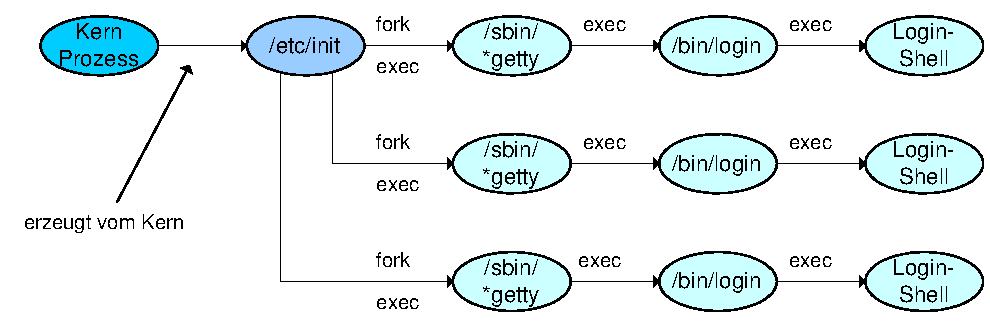
\includegraphics[width=10cm]{./files/inc/pictures/pdf/initprocess}
\caption{\label{pic:initprocess}Prozessvergabelung beim Start des Systems.}
\end{center}
\end{figure}

Man sieht, dass der init Prozess \verb~/sbin/*getty~ startet, was zu einer Reihe von *getty Prozessen\index{Prozesse unter Linux!getty} f�hrt. Jeder *getty Prozess stellt ein tty zu Verf�gung, das als erstes eine Begr�ssungsmeldung auf den Bildschirm schreibt (\verb~/etc/issue~) und anschliessend das login Programm (\verb~/bin/login~) startet. Dabei entsteht kein neuer Prozess. Das login Programm fordert den Benutzer auf, seinen Benutzernamen und das Passwort einzugeben. Dieser Ablauf wird im Folgenden noch genauer erkl�rt. Sobald das erfolgreich abgeschlossen ist, wird eine shell gestartet, die dem Benutzer weitere Eingaben erm�glicht.

\subsection{PAM - Pluggable Authentication Module}\index{PAM|textbf}
Was passiert nun genau, wenn das login Programm gestartet wurde und sich ein Benutzer anmeldet? Klassischerweise passiert folgendes:
\begin{itemize}
	\item Das login Programm\index{Login Programm} stellt durch Abfrage von Benutzernamen und Passwort sicher, dass der Benutzer �berhaupt exisiert und auch derjenige ist, der er vorgibt zu sein. Ferner werden im Erfolgsfalle dem Benutzer Gruppenrechte oder andere Privilegien gestattet.
	\item Es wird �berpr�ft, ob das Benutzerkonto �berhaupt g�ltig ist.
	\item Der Inhalt von \verb~/etc/motd~ wird auf dem Bildschirm ausgegeben. Danach wird ein Dienst zur Verf�gung gestellt. Dies ist in den meisten F�llen eine shell, kann aber auch ein anderer Dienst sein.
\end{itemize}
Damit ist eigentlich alles in Ordnung und man fragt sich, warum kompliziertere Authentifizierungsmechanismen wie PAM �berhaupt gebraucht werden.

Mit der klassichen Methode m�ssen die Authentisierungsmethoden in jedem Programm separat implementiert werden. Was macht man nun, wenn man die Anmeldung bei \emph{allen} Diensten durch ein anderes Verfahren austauschen m�chte? Man m�sste das Anmeldeverfahren bei allen Programmen neu implementieren und diese neu installieren. PAM (Pluggable Authentication Module) dient nun dazu, diese Authentisierungsmethoden zu vereinheitlichen. Das heisst, anstatt irgendein Anmeldeverfahren in einen Dienst-Server einzubauen, gibt dieser Dienst-Server die Aufgabe an die PAM-Bibliothek weiter. Diese wiederum liest die Konfigurationsdatei des Dienstes, und entscheidet dann, welche Verfahren in welcher Reihenfolge f�r die Anmeldung des Benutzers angewendet werden. Die verschiedenen Verfahren sind in den Modulen implementiert, die in der Konfigurationsdatei angegeben werden m�ssen. Dabei wird an die aufrufende Anwendung nur das Gesamtergebnis zur�ckgegeben. Dieses Prinzip ist in Abbildung \ref{pic:archpam} illustriert. Damit kann ein Administrator f�r jedes Programm (vom Netzwerk-Serverdienst �ber das Login bis hin zum Passwortgesch�tzten Bildschirmschoner) festlegen, welches Modul in welcher Reihenfolge abgearbeitet wird und was f�r einen Einfluss Erfolg oder Misserfolg eines Moduls auf den Anmeldevorgang haben.

\begin{figure}[h!tb]
\begin{center}
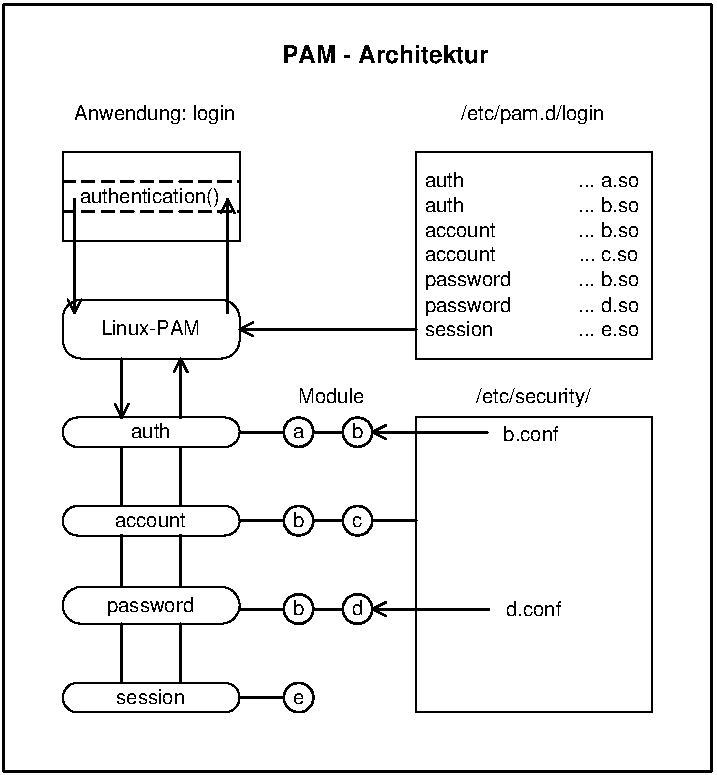
\includegraphics[width=8cm]{./files/inc/pictures/pdf/archpam}
\caption{\label{pic:archpam}Architektur des Pluggable Authentication Module}
\end{center}
\end{figure}

Es gibt f�r jedes Programm, dass PAM unterst�tzt im Verzeichnis \verb~/etc/pam.d/~ eine eigene Konfigurationsdatei\index{PAM!Konfigurationsdatei}, in der genau das Anmeldeverfahren f�r dieses Programm festgelegt werden kann. Hier ein Beispiel einer Konfigurationsdatei f�r das login Programm (\verb~/etc/pam.d/login~):
\begin{verbatim}
#%PAM-1.0
auth     required   /lib/security/pam_securetty.so
auth     required   /lib/security/pam_stack.so service=system-auth
auth     required   /lib/security/pam_nologin.so
account  required   /lib/security/pam_stack.so service=system-auth
password required   /lib/security/pam_stack.so service=system-auth
session  required   /lib/security/pam_stack.so service=system-auth
session  optional   /lib/security/pam_console.so
\end{verbatim}
Das Format ist immer wie folgt:
\begin{verbatim}
PAM-Dienst Wichtigkeit Modul Argumente
\end{verbatim}

\begin{description}
	\item[PAM-Dienst] Der Dienst beschreibt, welche Aufgabe das Modul im Anmeldevorgang �bernimmt.
	\begin{description}
		\item[auth] �bernimmt bei der Benutzeranmeldung zwei Aufgaben: Erstens wird der Benutzer �berpr�ft und zweitens werden Gruppenrechte (unabh�ngig von \verb~/etc/group~) oder andere Rechte vergeben.\index{PAM!auth@\texttt{auth}}
		\item[account] begrenzt den Zugang nach Folgenden Kriterien\index{PAM!account@\texttt{account}}
		\begin{itemize}
			\item Uhrzeit
			\item verf�gbare Systemressourcen (CPU, Speicher, etc.)
			\item Ort, von dem aus die Anmeldung statt findet.
		\end{itemize}
		\item[session] �bernimmt Aufgaben, die bevor oder nachdem der Benutzer den Dienst in Anspruch nimmt, hat ausgef�hrt werden sollen (z.B. log-Datei schreiben, Variablen setzen, etc.).\index{PAM!session@\texttt{session}}
		\item[password] wird aufgerufen, wenn ein Benutzer seinen Zugangscode �ndern will. Ein Zuganscode kann z.B. ein Passwort, ein Fingerabdruck oder �hnliches sein.\index{PAM!password@\texttt{password}} 
	\end{description}
	\item[Wichtigkeit] bestimmt, was f�r eine Bedeutung Erfolg bzw. Misserfolg der Anmeldung haben.
	\begin{description}
		\item[required] heisst, das Modul ist Notwendig. Schl�gt dieses fehl, schl�gt die gesamte Anmeldung fehl. Die folgenden Module werden aber dennoch abgearbeitet, um m�glichst viel �ber einen potentiellen Angreifer zu erfahren und ihm m�glichst wenig Anhaltspunkte �ber den Grund des Scheiterns zu geben.
		\item[requisite] wie required, jedoch bricht der Anmeldevorgang sofort ab.
		\item[sufficient] bedeutet, dass der Erfolg dieses Moduls f�r eine erfolgreiche Anmeldung ausreicht, falls vorher kein required-Modul fehlgeschlagen hat.
		\item[optional] hat keinen Einfluss auf den Anmeldevorgang, ausser, wenn \emph{nur} optional-Module in der Datei stehen.
	\end{description}
	\item[Modul und Argumente] beschreiben, welche Module f�r welche Aufgaben in welcher Reihenfolge verwendet werden.
\end{description}
Wie man sieht, ist PAM ein sehr m�chtiges Werkzeug und ein zentraler Mechanismus der Sicherheit. Die gegebene Beschreibung ist eine Einf�hrung. Es gibt sehr detaillierte Dokumentationen zu PAM. Diese k�nnen vom Web \cite{pam} heruntergeladen werden.

Im den vorhergehenden Abschnitten war immer die Rede vom \textit{login} Programm. PAM ist aber keineswegs auf dieses Programm beschr�nkt. Wie schon erw�hnt, kann PAM in Verbindung mit jedem Programm, das PAM unterst�tzt, verwendet werden.



	\chapter{Software}
\label{cha:Software}
\index{Software}
In diesem Kapitel wird der theoretische Hintergrund von Einstelleungen und Optionen von den Softwareprodukten erl�utert, die f�r den Versuch ben�tigt werden. Dabei werden nur die Optionen erkl�rt, denen eine besondere Bedeutung im Zusammenhang mit den �bungen zukommt.
%----------
\section{PitBull}
\label{sec:PitBull}
\index{PitBull}
PitBull eine Software von der Firma Argus Systems Group erm�glicht eine zus�tzliche Sicherung des Systems. Herausragendster Vorteil der zus�tzlichen Sicherung eines Systems durch PitBull ist der Schutz vor Sicherheitsl�chern in installierten Softwarekomponenten. Zum Beispiel w�rde sie, wenn der Angreifer mit einer Bufferoverlow Attacke die Rechte des angegriffenen Dienstes erh�lt verhindern, dass er weiter ins System eindringen kann.

In den �bungsaufgaben kommt PitBull nicht zum Einsatz, da in der zur Verf�gung stehenden Zeit nicht gen�gend aussagekr�ftige Beispiele zur Demonstration der Eigenheiten eines mit PitBull gesicherten Systems gefunden werden konnten. Mehr zu diesem Entscheid ist im Anhang \ref{cha:EvaluationDesUebungsablaufs} "`Evaluation des �bungsablaufs"' auf Seite \pageref{cha:EvaluationDesUebungsablaufs} zu lesen.
%----------
\section{Rlogin}
\index{rlogin@\texttt{rlogin}}
\label{sec:rlogin}
Mit rlogin ist es m�glich sich bei einem System anzumelden (�hnlich wie mit telnet). Dazu ist es notwendig, dass auf dem System der Dienst rlogind gestartet wurde. Die Syntax f�r den Befehl lautet:\\ \verb~rlogin -l {Benutzername} {Hostname oder IP-Adresse}~\\Befindet sich auf dem System, auf welchem der Dienst gestartet im Verzeichnis eines Benutzers eine Datei namens \verb~.rhosts~, so kann sich dieser Benutzer von den Systemen, die in dieser Datei eingetragen sind ohne Passwort anmelden. M�glicher Inhalt der Datei \verb~.rhosts~:
\begin{verbatim}
					192.168.0.1 master
					192.168.0.3 master
\end{verbatim}
Befindet sich diese Datei im \verb~home~-Verzeichnis des Benutzers \verb~master~ kann dieser Benutzer von den IP-Adressen 192.168.0.1 und 192.168.0.3 ohne Passwort auf das System zugreifen.
Das Deaktivieren oder Aktivieren dieses Dienstes geschieht unter Red Hat durch Editieren der Datei \verb~\etc\xinetd.d\rlogin~. Dies ist ein Beispiel f�r den Inhalt der Datei:
\begin{verbatim}
# default: on
# description: rlogind is the server for the rlogin(1) program. \
# The server \
# provides a remote login facility with authentication based on \
# privileged port numbers from trusted hosts.
service login
{
	socket_type		= stream
	wait			= no
	user			= root
	log_on_success		+= USERID
	log_on_failure 		+= USERID
	server			= /usr/sbin/in.rlogind
	disable			= no 
}
\end{verbatim}
In der abgebildeten Konfigurationsdatei ist der \verb~rlogin~-Dienst eingeschaltet. Dies ist zu sehen an der Zeile \verb~disabled=no~. Wird die Zeile durch den Eintrag \verb~disabled=yes~ ersetzt, ist der Dienst ausgeschaltet.
%-----------
\section{Arp}
\index{arp@\texttt{arp}}
\label{sec:arp}
Der Befehl \verb~arp~ erlaubt es den Arp-Cache anzuzeigen oder zu konfigurieren. Mit dem Parameter -a kann der Arp-Cache angezeigt werden. Mit der Syntax\\ \verb~arp -s {IP-Adresse} {MAC-Adresse}~\\ kann f�r eine IP-Adresse eine statische MAC-Adresse gesetzt werden. Dies ist eine M�glichkeit, um zu verhindern, dass dem System eine falsche MAC-Adresse untergeschoben wird.
%-----------
\section{Finger}
\index{finger@\texttt{finger}}
\label{sec:finger}
�ber den Befehl \verb~finger~ k�nnen Informationen �ber die Benutzer eines Systems abgefragt werden, falls auf dem System der entsprechende Dienst gestartet wurde. Um die momentan an einem System angemeldeten Benutzer anzuzeigen benutzt man den Befehl mit der Syntax \verb~finger @{Hostname oder IP-Adresse}~. Um Detailinformationen �ber einen Benutzer des Systems zu erhalten kann vor dem @-Zeichen der Benutzer angegeben werden.
Die Deaktivierung oder Aktivierung dieses Dienstes erfolgt analog zum Dienst \verb~rlogin~ aus dem Abschnitt \ref{sec:rlogin}. Die Konfigurationsdatei des \verb~finger~-Dienstes lautet \verb~\etc\xinetd.d\finger~. Ist der Dienst aktiviert sieht sie folgendermassen aus:
\begin{verbatim}
# default: on
# description: The finger server answers finger requests. Finger is \
#	a protocol that allows remote users to see information such \
#	as login name and last login time for local users.
service finger
{
	socket_type	= stream
	wait		= no
	user		= nobody
	server		= /usr/sbin/in.fingerd
	disable		= no
}
\end{verbatim}
%----------
\section{VMware}
\label{sec:Vmware}
In diesem Kapitel geht es um ausgew�hlte Themen zur Benutzung und Installation eines VMware Systems. Im Besonderen werden die Themen genauer erl�utert, die im Ramen des Einrichtens der �bungsumgebung besonderer Aufmerksamkeit bed�rfen. Eine konkrete Anleitung zur Installation ist im Kapitel \ref{cha:Installation} auf Seite \pageref{cha:Installation} zu finden.
\subsection{Begriffe}
\label{sub:Begriffe}
Im Folgenden wird der Begriff \emph{VMware Host} oder \emph{Host System} verwendet werden. Damit wird das System bezeichnet auf welchem VMware installiert wird (Im Ramen dieser Arbeit ist dies ein Linux System mit Red Hat 7.3).

Unter dem \emph{virtuellen System} (auch \emph{Virtual Machine}) wird das System verstanden, das innerhalb der VMware Umgebung l�uft. Dem virtuellen System werden Hardwarekomponenten vorgespielt. Die VMware Umgebung leitet die Anfragen auf diese simulierten Hardwarekomponenten weiter auf reale Hardwarekomponenten des Host Systems. Es gibt verschiedene M�glichkeiten das Betriebssystem f�r das virtuelle System aufzusetzen. Entweder es existiert bereits eine reale Harddisk mit einem bereits vollfunktionsf�higen Betriebssystem oder es wird von VMware eine virtuelle Disk erzeugt, auf die, nach dem Booten des virtuellen Systems das gew�nschte Betriebssystem installiert werden kann (Option \emph{virtual disk}). Im ersten Fall ist nur der Ort an dem sich das bereits lauff�hige Betriebssystem befindet anzugeben.
Vollst�ndigkeitshalber sollte hier erw�hnt werden, dass es noch eine weitere M�glichkeit gibt ein virtuelles System mit einem Betriebssystem auszur�sten. Die Firma VMware stellt sogenannte VMware Guest OS Kit's zur Verf�gung, dies sind f�r VMware vorkonfigurierte Betriebssysteme.
\subsection{Diskmodi von Virtuellen Disks}
\label{subsec:Diskmodi}
\index{Diskmodi}
\index{Virtual Disk}
Einem virtuellen System kann Speicherplatz in Form von virtuellen Disks zugeordnet werden. F�r diese Disks existieren drei verschiedene Modi: \emph{Persistent},\emph{Undoable} und \emph{Nonpersistent}. Diese Modi bestimmen, wie die Daten der Disks gespeichert werden. Einem virtuellen System k�nnen mehrere virtuelle Disks zur Verf�gung gestellt werden.
\subsubsection{Persistent}
\index{persistent}
Die virtuelle Disk verh�lt sich wie eine physische Harddisk: Daten werden nachdem sie ge�ndert wurden sofort gespeichert. Der Zustand der Disks bleibt nach einem Neustart des virtuellen Systems erhalten.
\subsubsection{Undoable}
\index{undoable}
�nderungen auf der virtuellen Disk werden in einer Datei (mit der Namenserweiterung \verb~.REDO~)  protokolliert und k�nnen beim Herunterfahren des virtuellen Systems r�ckg�ngig oder definitiv gemacht werden.
\subsubsection{Nonpersistent}
\index{nonpersistent}
Die Datei der virtuellen Disk wird nur gelesen. �nderungen der Daten werden wie bei \emph{undoable} protokolliert. Die �nderungen auf der virtuellen Disk werden beim Herunterfahren automatisch r�ckg�ngig gemacht. 
\subsection{Duplizieren eines virtuellen Systems}
\label{DuplizierenEinesVirtuellenSystems}
\index{Virtuelles System!duplizieren}
\index{Virtual Disk!kopieren}
Hier wird davon ausgegangen, dass beim Erstellen des virtuellen Systems mit der Option \emph{virtual disk} gearbeitet wurde (Abschnitt \ref{sub:Begriffe} auf Seite \pageref{sub:Begriffe}).
F�r jedes virtuelle System wird ein eigenes Verzeichnis erstellt. In diesem Verzeichnis befinden sich alle relevanten Daten. Im VMWare Handbuch \cite{VMwareManual} wird empfohlen vor dem Ver�ndern der Dateien eines virtuellen Systems vom gesamten Verzeichnis ein Backup anzulegen. Um ein virtuelles System zu duplizieren braucht man bloss dieses Verzeichnis zu kopieren. Dazu muss das virtuelle System heruntergefahren werden. Falls zus�tzliche Dateien ausserhalb des Verzeichnisses erstellt wurden, die das virtuelle System benutzt, m�ssen diese vom neuen Verzeichnis aus �ber die gleichen relativen Pfade erreichbar sein.
Nun kann �ber den Men�punkt \verb~File > Open~ die Konfigurationsdatei des kopierten virtuellen Systems ge�ffnet werden, womit das soeben kopierte System geladen wird. 

Die Portierung eines virtuellen Systems von einem Linux Rechner auf einen Windows Rechner ist laut VMware Handbuch \cite{VMwareManual} auch m�glich.
\subsection{Netzwerkkonfiguration}
\label{subsec:Netzwerkkonfiguration}
\index{VMware!Netzwerkkonfiguration}
Beim Einrichten eines neuen virtuellen Systems kann man zwischen drei verschiedenen Netzwerkintegrationen w�hlen: \emph{Bridged}, \emph{Host-only} oder \emph{NAT}. Bei der Wahl eines Modus ist darauf zu achten, dass bei der Installation von VMware die Frage nach der Unterst�tzung des entsprechenden Modus best�tigt wurde. Sobald die Netzwerkunterst�tzung von VMware aktiviert wird, erstellt es virtuelle Switches\index{Virtueller Switch}. Diese sind im Host System als Netzwerkkomponenten zu erkennen. Es k�nnen bis zu zehn solche Switches erzeugt werden. Einige von ihnen tragen spezielle Bezeichnungen wie \emph{Bridged} (auch VMnet0), \emph{Host-only} (auch VMnet1) oder \emph{NAT} (auch VMnet8). Diese speziellen Switches werden in den entsprechenden Netzwerkkonfigurationen verwendet.\\
Ein virtuelles System kann an einen beliebigen, virtuellen Switch angeh�ngt werden. An einen virtuellen Switch k�nnen auch mehrere virtuelle Systeme angeh�ngt werden. Im Folgenden werden die verschiedenen Netzwerkintegrations Modi erkl�rt.
\subsubsection{Bridged Modus}
\label{subsubsec:BridgedModus}
\index{Bridged Modus}
Dieser Modus verbindet das virtuelle System mit dem LAN, an welchem das Host System angeschlossen ist. Falls das Host System �ber mehrere Netzwerkkarten verf�gt, k�nnen f�r diese auch mehrere Bridges definiert werden.
\begin{figure}[H]
\begin{center}
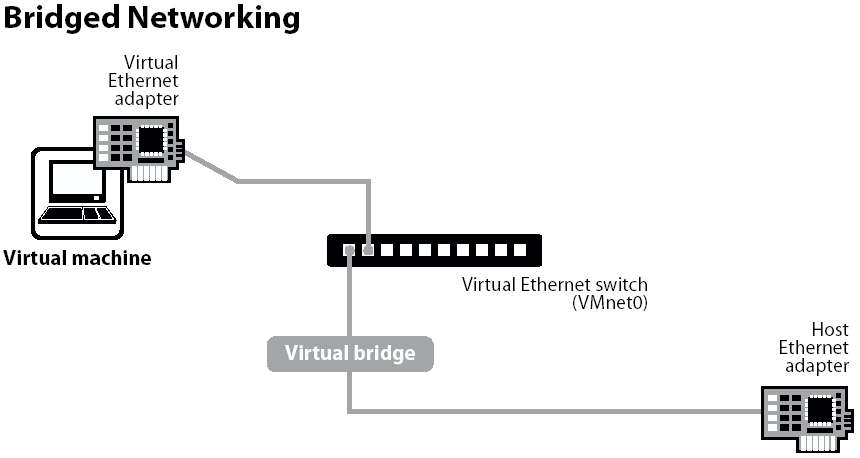
\includegraphics[width=13cm]{./files/inc/pictures/jpg/vmware_bridged.jpg}
\end{center}
\caption{\label{pic:bridgedmodus}Verbindung des virtuellen Systems �ber den Ethernetadapter des Hosts mit dem Netzwerk im Bridged Modus}
\end{figure}
Abbildung \ref{pic:bridgedmodus} (entnommen aus dem VMware Handbuch \cite{VMwareManual}) zeigt die Komponenten, die in diesem Modus simuliert werden und wie sie mit dem realen Host verbunden sind. Die einzige reale Komponente, die auf der Abbildung zu sehen ist, ist der Ethernetadapter des Host Systems (bezeichnet mit "`Host Ethernet adapter"'). Ein virtueller Netzwerkadapter ("`Virtual Ethernet adapter"') und ein virtueller Switch ("`Virtual Ethernet switch"') werden von VMware simuliert. Logisch ist das Host System �ber den virtuellen Switch mit dem virtuellen System verbunden. Diese Verbindung ist in der Abbildung mit "`Virtual bridge"' bezeichnet. Das System ist vergleichbar mit zwei realen Systemen, die an dem gleichen Switch angeschlossen sind. Andere Systeme, die mit dem Host System verbunden sind, sind logisch ebenfalls mit dem virtuellen Switch verbunden.
Die Wahl der IP-Adressen ist unabh�ngig von der VMware-Umgebung. Die IP-Adressen k�nnen so gew�hlt werden, wie sie auch f�r reale Netzwerkkomponenten gew�hlt w�rden. Zum Beispiel k�nnte die IP-Adresse des virtuellen Systems 192.168.0.101 und die des Hostsystems 192.168.0.1 lauten, falls sich die Systeme im gleichen Subnetz befinden sollen.
\subsubsection{Host-only Modus}
\label{subsec:HostOnlyModus}
\index{Host-only Modus}
In diesem Modus simuliert das virtuelle System dem Host System ein Interface mit der Bezeichnung Host-Only (VMware Linux) oder einen Ethernet Adapter (VMware Windows). Dieser Modus wird benutzt, falls das virtuelle System keine Verbindung zu einem realen Netzwerk, mit dem das Host System m�glicherweise verbunden ist, aufweisen soll.
\begin{figure}[H]
\begin{center}
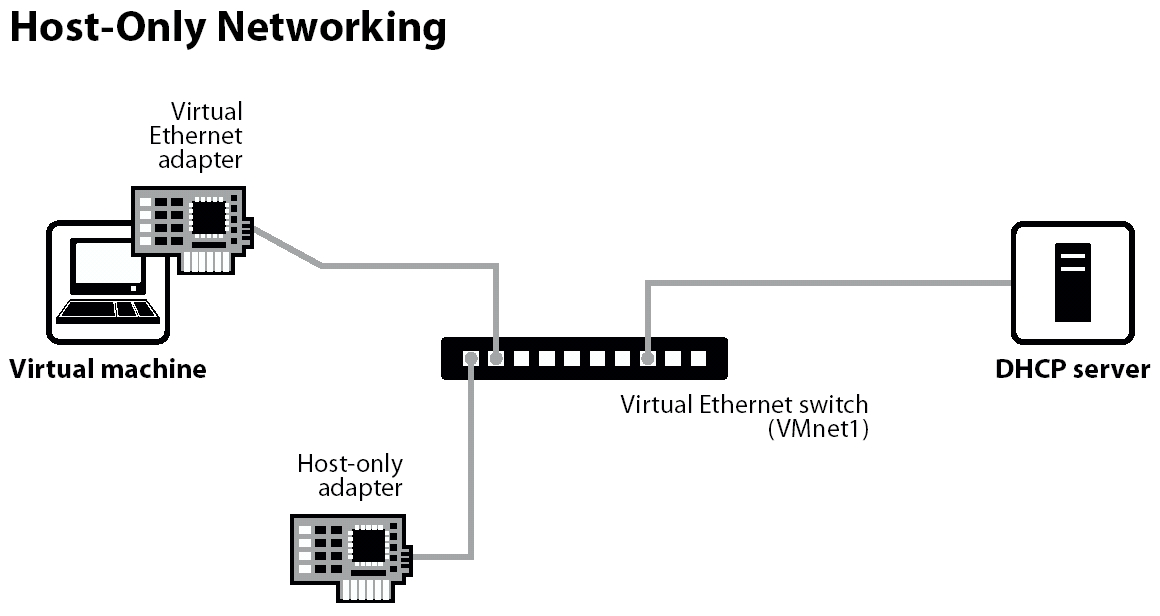
\includegraphics[width=13cm]{./files/inc/pictures/jpg/vmware_hostonly.jpg}
\end{center}
\caption{\label{pic:hostonlymodus}Im Host-only Modus simulierte Netzwerkkomponenten}
\end{figure}
Abbildung \ref{pic:hostonlymodus} zeigt die Komponenten, die in diesem Modus simuliert werden: Ein virtueller Netzwerkadapter ("`Virtual Ethernet adapter"'), ein virtueller Switch ("`Virtual Ethernet switch"') und ein DHCP Server. Der DHCP Server ordnet dem virtuellen System automatisch eine IP-Adresse zu. Das virtuelle System erh�lt keinen Zugang zum Netzwerk das mit dem Ethernetadabter des Host Systems verbunden ist, ausser es wird auf dem Host System eine entsprechende Software installiert (zum Beispiel ein Proxy Server). Ein Proxy Server k�nnte dann die Anfragen des virtuellen Systems, die er �ber den virtuellen Netzwerkadapter ("`Host-only adapter"') erh�lt �ber den realen Hostadapter des Host Systems in ein angeschlossenes Netzwerk weiterleiten. Das bedeutet auch, dass andere Rechner der gleichen Broadcastdomain wie das Host System nichts von dem Virtuellen System sehen, falls kein Proxy installiert ist.
\subsubsection{Network Address Translation (NAT) Modus\index{NAT Modus}}
\label{subsec:NATModus}
Die Installation des NAT Modus ist notwendig, falls f�r das virtuelle System keine eigene IP-Adresse zur Verf�gung steht. Falls das Host System per \emph{Wireless LAN} oder \emph{Dial-Up Verbindung} mit einem anderen Netzwerk verbunden ist, stellt der NAT Modus eine M�glichgkeit dar, wie das virtuelle System Zugriff zum Netzwerk erhalten kann, mit welchem das Host System verbunden ist. Das virtuelle System ist �ber die gleiche IP-Adresse wie das Host System erreichbar.
\begin{figure}[H]
\begin{center}
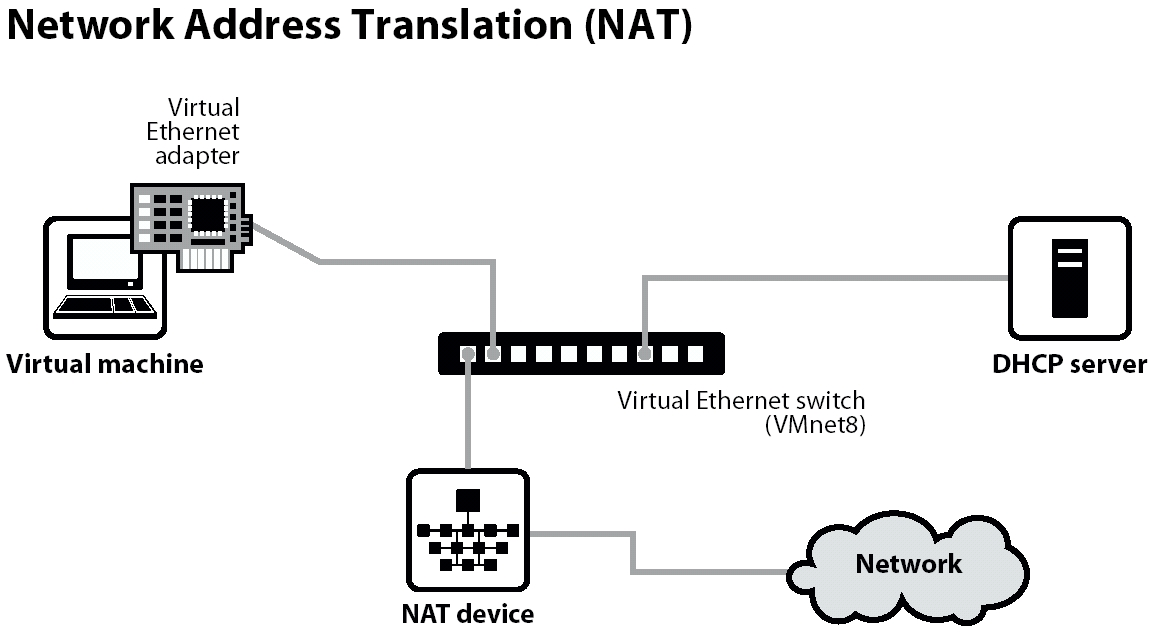
\includegraphics[width=12.5cm]{./files/inc/pictures/jpg/vmware_nat.jpg}
\end{center}
\caption{\label{pic:natmodus}Verbindung des virtuellen Systems �ber den Ethernetadapter des Hosts mit dem Netzwerk im NAT Modus}
\end{figure}
In Abbildung \ref{pic:natmodus} sind die simulierten Komponenten zu sehen: Ein virtueller Netzwerkadapter ("`Virtual Ethernet adapter"'), ein virtueller Switch ("`Virtual Ethernet switch"'), ein DHCP Server und ein sogenanntes \emph{NAT Device}. Das reale Netzwerk, an dem auch das Host System angeschlossen ist, ist mit "`Network"' gekennzeichnet. Logisch ist es direkt mit dem NAT Device verbunden. Das NAT Device erm�glicht es einem realen System, das an dem gleichen Netzwerk angeschlossen ist wie das Host System, mit dem virtuellen System zu kommunizieren. Die Angabe einer Portnummer erm�glicht es dem NAT Device zu entscheiden, ob mit der Adresse das Host System oder das virtuelle System gemeint ist. Der DHCP Server ordnet dem virtuellen System, auf dem nach aussen nicht sichtbaren Netz, automatisch eine IP-Adresse zu. 
\subsection{Tips und Tricks}
\subsubsection{Wechseln zwischen VMwarehost und virtuellem System}
L�uft ein virtuelles System, erh�lt man per \verb~Ctrl + Alt~ die Kontrolle �ber das Hostsystem. Diese spezielle Tastenkombination ist n�tig, weil alle anderen Eingaben von der virtuellen Konsole interpretiert werden. Um wieder das virtuelle System zu steuern braucht man nur in das Fenster der VMware Applikation zu klicken.
\subsubsection{Installation eines virtuellen RedHat Systems}
Bei der Installation von RedHat auf einem virtuellen System ist es empfehlenswert die  Installation im textbasierten Modus durchzuf�hren. Die Bedienung der grafikbasierten Installation ist aus Gr�nden der Geschwindigkeit etwas m�hsam.
\subsubsection{Hinweis bez�glich VMware Tools Package}
\index{VMware Tools Package}
Beim Start des virtuellen Systems wird ein Hinweis angezeigt, dass \emph{VMware Tools} installiert werden m�sse. Dies ist f�r die Installation von virtuellen Servern jedoch nicht notwendig, da keine speziellen Grafikfunktionen verwendet werden. \emph{VMware Tools} w�rde es beispielsweise erm�glichen eine h�here Aufl�sung als 640x480 mit 16 Farben zu verwenden.
\subsubsection{CD Wechsel bei der Installation des virtuellen Servers}
\index{Fehler!CD-Wechseln}
\begin{verbatim}
The CD-ROM drive failed to eject the disc with the error:
Device or resource busy.
\end{verbatim}
Um dieses Problem zu beheben hilft es das CD-Rom Laufwerk ausserhalb von VMware zu unmounten und wieder zu mounten. Der Fehler und die Behebung konnte aber nicht repliziert werden.

\subsection{Erfahrungen}
\subsubsection{Kopieren einer Virtual Disk}
\index{Fehler!Kopieren einer Virtual Disk}
Das gesamte Verzeichnis eines virtuellen Systems wurde kopiert. Nach dem Starten des kopierten Systems sollte auf dem virtuellen System Pitbull isntalliert werden. Nach der Initierung des Installationsskriptes von Pitbull gab es eine Fehlermeldung begleitet von Steuerzeichen, die auf Probleme der Festplatte hinwiesen. Die Meldung wurde in der Konsole angezeigt, in welcher gerade das Installationsskript ausgef�hrt wurde. Da das Skript gerade auf eine Eingabe wartete ist es wahrscheinlich, dass das Betriebssystem die Meldung erzeugte und dass es ein Problem mit dem Zugriff auf den virtuellen Disk gab. Merk�rdigerweise schien dieser Zugriffsfehler das VMware Hostsystem beeintr�chtigt zu haben.

Das Home-Verzeichnis des VMware Benutzers wies anschliessend ung�ltige Ver\-zeichnis- und Dateinamen auf (siehe Abbildung \ref{pic:scrambledfat}).
\begin{figure}[H]
\begin{center}
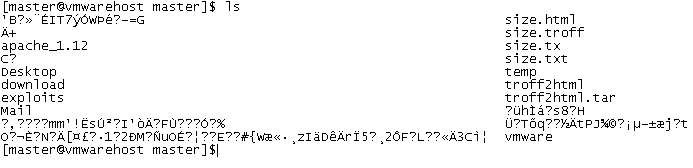
\includegraphics[width=14cm]{./files/inc/pictures/jpg/scrambledfat.jpg}
\end{center}
\caption{\label{pic:scrambledfat}Ausgabe des ls-Commandos mit defekten Dateieintr�gen}
\end{figure}
Das System war immer noch funktionst�chtig. Die erstellten Dateien haben keinerlei Inhalt und k�nnen ohne Beeintr�chtigung des Systems gel�scht werden.


%\part{Testing}
%\label{par:Testing}

\part{Lab}	
\label{par:Lab}
\vspace{2cm}
Der folgende Teil enth�lt eine Beschreibung zur Installation der �bungsumgebung, sowie die �bungsaufgaben und deren L�sungen.
%	\input{./files/uebungsbeschreibung}
	\chapter{Installation der �bungsumgebung\index{Installation der �bungsumgebung}}
\label{cha:Installation}
Das folgende Kapitel beschreibt, wie die �bungsumgebung aufgebaut werden kann. Die schnellste Methode um eine lauff�hige �bungsumgebung zu erhalten ist, das Installieren der Software VMware und dem Kopieren und Starten der virtuellen Disks (siehe "`Dublizieren eines virtuellen Systems"' in Abschnitt \ref{DuplizierenEinesVirtuellenSystems} auf Seite \pageref{DuplizierenEinesVirtuellenSystems}). Auf den beiliegenden CDs befinden sich die Dateien der virtuellen Disks der Server 1 und 2 (siehe Anhang \ref{cha:BeiliegendeCds}).
%----------
\section{VMware Hostsystem\index{Installation der �bungsumgebung!VMware Hostsytem}}
\label{sec:VmwareHostsystem}
\index{Hostsystem}
Das VMware Hostsystem, ist das System auf dem VMware gestartet wird. F�r die Installation des VMware Hostsystems wurde Red Hat 7.3 verwendet\footnote{Da die Software VMware auch f�r das Betriebssystem Windows erh�ltlich ist, k�nnte f�r das VMware Hostsystem der �bungsumgebung auch ein System mit Windows benutzt werden.}. Es wurde eine Standard Installation eines Desktop-Systems mit Netzwerkzugang durchgef�hrt. F�r die graphische Oberfl�che wurde X-Windows mit dem Window Manager KDE, in den Versionen die mit diesem Release mitgeliefert werden installiert. W�hrend der Installation wurden folgende Einstellungen in der angegebenen Reihenfolge vorgenommen. Bei nicht angegebenen Optionen wurde die Standardeinstellung beibehalten.
\begin{itemize}
\item textbasierte Installation durch die Eingabe von \verb~text~ w�hlen
\item Sprache f�r den Installationsvorgang: Deutsch
\item Tastaturtyp: sg-latin1
\item Maustyp: Microsoft IntelliMouse (PS/2), ohne die Drei-Tastentyp-Emulation
\item \textbf{Installationstyp: Desktop}
\item F�r die Partionierung wurde der \emph{Disk Druid} gew�hlt.
\item Initialisierung und L�schen des Disks best�tigen (es handelt sich hierbei, um die virtuelle Harddisk)
\item \textbf{Partitionen: 47MB (ext3) /boot ,604 MB (swap), / (ext3) 5498MB}\index{Installation der �bungsumgebung!partitionieren} (hier kann die Gr�sse auf 1 MB eingestellt und die Option "`Den gesamten verf�gbaren Platz ausf�llen"' selektiert werden.
\item Bootloader GRUB ausw�hlen
\item Bootloader im Masterboot record installieren lassen
\item Keine speziellen Boot-Optionen eintragen
\item kein GRUB Passwort verwenden
\item Die Optionen "`bootp"'und "`dhcp"' deaktivieren, IP-Adresse \textbf{(z.B. 192.168.0.2)} und Netzmaske (z.B. 255.255.255.0) eintragen\footnote{Falls das Hostsystem mit den Virtuellen Servern kommunizieren m�chte, muss seine IP-Adresse aus dem gleichen Subnetz, wie die IP-Adresse des virtuellen Servers(siehe Abschnitt \ref{sec:VirtuellesSystem} "`Virtuelles System"') stammen. Ansonsten kann die IP-Adresse frei gew�hlt werden.}
\item als Rechnername zum Beispiel "`\textbf{vmwarehost}"' 
\item keine Firewall selektieren
\item "`German Switzerland"' selektieren (auch als standard Sprache)
\item Zeitzone Europa/Z�rich
\item Root \textbf{Passwort : hard2go}
\item neuer User erstellt, \textbf{User: master}, \textbf{Passwort: behave}
\item keine zus�tzlichen Pakete selektiert
\end{itemize}
Der ben�tigte Speicherplatz f�r diese Installation bel�uft sich auf 915MB. Ein vollst�ndiges Protokoll der Installation ist unter \verb~/root/install.log~ zu finden.
Erkl�rungen zu den einzelnen Optionen und weitere Installationsdetails k�nnen den Online Handb�chern von RedHat entnommen werden (Installation von Red Hat 7.3 \cite{installLinux73} oder f�r die aktuelleste Version \cite{installLinuxCurrent}).
%----------
\section{Virtuelles System\index{Installation der �bungsumgebung!Virtuelles System}}
\label{sec:VirtuellesSystem}
Wie in der Evaluation des �bungsablaufs im Anhang \ref{cha:EvaluationDesUebungsablaufs} auf Seite \pageref{cha:EvaluationDesUebungsablaufs} erl�utert werden f�r die �bung mit VMware zwei Server simuliert: Server 1 und Server 2. In den folgenden Abschnitten wird erkl�rt, wie in VMware die zu simulierenden Hardwarekomponenten eingestellt werden und anschliessend die beiden Server innerhalb der VMware-Umgebung aufgesetzt werden.
\subsection{VMware Konfiguration\index{VMware!Konfiguration}}
\label{subsec:VmwareKonfiguration}
Die Installation eines virtuellen Servers erfolgt nach dem Starten von VMware am einfachsten �ber den "`Configuration Wizard"'. Die einstellbaren Optionen sind gut beschrieben. Um ein neues Virtuelles System aufzusetzten sind folgende Einstellungen in der hier aufgez�hlten Reihenfolge zu machen.
\begin{itemize}
\item Create standard virtual machine
\item Linux
\item \emph{Display name} Bsp. "`Standard Server"'
\item "`Full path of the virtual machine directory"' \\Bsp.			\verb~/home/master/vmware/standard_server/~
\item Create a new virtual disk
\item "`Virtual disk size (in megabytes)"' Bsp. 1300
\item CD-ROM: Standard-Einstellungen belassen
\item Floppy: Standard-Einstellungen belassen
\item Bridged networking (\emph{Bridged Modus} in Kapitel \ref{subsec:Netzwerkkonfiguration} auf Seite \pageref{subsubsec:BridgedModus})
\end{itemize}
Bemerkung: Der Hauptspeicher wird standardm�ssig mit 32 MB eingerichtet. Falls mehr Hauptspeicher zur Verf�gung steht, kann dies nach Beenden des "`Wizards"' auf folgende Weise eingestellt werden:
\begin{enumerate}
\item �ber \verb~Settings>Configuration Editor~ den Konfigurationseditor �ffnen
\item In der Auflistung von Systemkomponenten "`Memory"' ausw�hlen
\item Den Wert von "`Guest Size (MB)"' auf \verb~128~ einstellen
\end{enumerate}
Nun ist die virtuelle Hardware des zu simulierenden Servers eingstellt. Jetzt kann auf dem virtuellen System ein Betriebssystem installiert werden.  

\subsection{Virtuelle Server\index{Installation der �bungsumgebung!Virtuelles System!Virtuelle Server}}
\index{Installation!Server 1}
\index{Installation!Server 2}
\label{subsec:VirtuelleServer}
Um auf dem virtuellen System Linux zu installieren, muss die erste CD der Distribution eingelegt und das virtuelle System gestartet werden. Dies geschieht �ber die "`Power On"' Schaltfl�che. Das virtuelle System wird direkt von der realen CD gestartet. Alternativ k�nnte das Betriebssystem auch von ISO Image-Dateien der CDs erstellt werden (siehe VMWare Handbuch 
\cite{VMwareManual}).

F�r die Installation der beiden virtuellen Server wurde Red Hat 7.3 verwendet. Der Installationsvorgang der beiden Server unterscheidet sich nur darin, das bei Server 1 w�hrend der Installation die Option "`Shadow-Passw�rter verwenden"' deaktiviert wird. Im folgenden wird in den einzelnen Schritten des Installationsvorgangs darauf hingewiesen, wenn f�r die Server eine individuelle Einstellung notwendig ist. Auf den Servern wird keine graphische Oberfl�che installiert. W�hrend der Installation werden folgende Einstellungen in der angegebenen Reihenfolge vorgenommen. Bei nicht angegebenen Optionen ist die Standardeinstellung beizubehalten.
\begin{itemize}
\item textbasierte Installation durch die Eingabe von \verb~text~ w�hlen
\item Sprache f�r den Installationsvorgang: Deutsch
\item Tastaturtyp: sg-latin1
\item Maustyp: Microsoft IntelliMouse (PS/2), ohne die Drei-Tastentyp-Emulation
\item
	Server 1: \textbf{Installationstyp: Benutzerdefinierte Installation}\footnote{Standardm�ssig w�rde sonst Password-Shadowing installiert werden.}
	\\Server 2: \textbf{Installationstyp: Server}
\item F�r die Partionierung wurde der \emph{Disk Druid} gew�hlt.
\item Initialisierung und L�schen des Disks best�tigen (es handelt sich hierbei, um die virtuelle Harddisk)
\item \textbf{Partitionen: 47MB (ext3) /boot ,200 MB (swap), / (ext3) 1052MB}\index{Installation der �bungsumgebung!partitionieren} (hier kann die Gr�sse auf 1 MB eingestellt und die Option "`Den gesamten verf�gbaren Platz ausf�llen"' selektiert werden.
\item Bootloader GRUB ausw�hlen
\item Bootloader im Masterboot record installieren lassen
\item Keine speziellen Boot-Optionen eintragen
\item kein GRUB Passwort verwenden
\item Die Optionen "`bootp"'und "`dhcp"' deaktivieren\footnote{Die IP-Adresse wird manuell gesetzt, darum wird der DHCP-Dienst nicht ben�tigt.}\index{Installation der �bungsumgebung!IP-Adressen}
	\\Server 1: \textbf{IP-Adresse 192.168.0.100}\footnote{Der Versuch ist nicht abh�ngig von den gew�hlten IP-Adressen. Diese IP-Adressen sind als Vorschl�ge zu verstehen.}
	\\Server 2: \textbf{IP-Adresse 192.168.0.200}\\
	Netzmaske 255.255.255.0 eintragen
\item als Rechnername zum Beispiel "`server1"', beziehungsweise "`server2"'
\item keine Firewall selektieren
\item "`German Switzerland"' selektieren (auch als standard Sprache)
\item Zeitzone Europa/Z�rich
\item Root \textbf{Passwort : hard2go}
\item neuer User erstellt,\textbf{ User: master},\textbf{ Passwort: behave}
\item Konfigurationansicht der Authentifizierung (betrifft nur Server 1): Die Option "`Shadow-Passw�rter verwenden"' deaktivieren
\item alle Pakete deselektiert, Web-Server selektiert
\end{itemize}
Diese Installation ben�tigt 940 MB Speicherplatz auf dem virtuellen System. Ein vollst�ndiges Protokoll der Installierten Pakete wird sp�ter unter \verb~/root/install.log~ zu finden sein.
Die Ausgabe des Befehls \verb~ifconfig~\index{ifconfig@\texttt{ifconfig}} auf dem virtuellen System liefert uns die folgende Informationen\footnote{Falls die Ausgabe nicht den Erwartungen entspricht, k�nnen die Netzwerkeinstellungen zum Beispiel mit dem Konfigurationsprogramm \verb~/usr/bin/setup~\index{setup@\texttt{setup}} editiert werden}:
\begin{figure}[H]
\begin{center}
\begin{verbatim}
eth0      Protokoll:Ethernet  Hardware Adresse 00:50:56:40:00:46  
          inet Adresse:192.168.0.100  Bcast:192.168.0.255
          Maske:255.255.255.0
          UP BROADCAST RUNNING MULTICAST  MTU:1500  Metric:1
          RX packets:14 errors:0 dropped:0 overruns:0 frame:0
          TX packets:12 errors:0 dropped:0 overruns:0 carrier:0
          Kollisionen:0 Sendewarteschlangenl�nge:100 
          RX bytes:1425 (1.3 Kb)  TX bytes:1354 (1.3 Kb)
          Interrupt:10 Basisadresse:0x10a0 
          
lo        Protokoll:Lokale Schleife  
          inet Adresse:127.0.0.1  Maske:255.0.0.0
          UP LOOPBACK RUNNING  MTU:16436  Metric:1
          RX packets:8 errors:0 dropped:0 overruns:0 frame:0
          TX packets:8 errors:0 dropped:0 overruns:0 carrier:0
          Kollisionen:0 Sendewarteschlangenl�nge:0 
          RX bytes:560 (560.0 b)  TX bytes:560 (560.0 b)
\end{verbatim}



\caption{Ausgabe des Befehls ifconfig auf dem virtuellen System\label{pic:ifconfig}}
\end{center}
\end{figure}
In der Abbildung \ref{pic:ifconfig} ist zu erkennen, dass das virtuelle System eine IP-Adresse und eine MAC-Adresse erhalten hat. Die Ausgabe ist nicht zu unterscheiden von einem realen System mit einer realen Netzwerkkarte. Nun kann auf einem anderen Rechner des Uebungsnetzes in einem Browser die IP-Adresse (hier 192.168.0.100) eingegeben werden und es wird eine Standard Webseite des Apache-Webservers angezeigt.

Auf dem Server 1 werden nach der Installation die Dienste \verb~rlogin~ und \verb~finger~ aktiviert. Wie diese Dienste aktiviert werden entnehmen sie bitte dem Abschnitt \ref{sec:rlogin} zum Thema \verb~rlogin~ auf Seite \pageref{sec:rlogin} und dem Abschnitt \ref{sec:finger} zum Thema \verb~finger~ auf Seite \pageref{sec:finger}.

Auf Server 2 sind die Dienste \verb~finger~ und \verb~rlogin~ deaktiviert. Das Bootmanagerpasswort ist eingschaltet und lautet: \textbf{nashorn}. Wie der Bootmanager GRUB konfiguriert werden muss, um das Bootmanagerpasswort zu aktivieren ist in den L�sungen zu den �bungen in Abschnnitt  \ref{sec:Loesungen} auf Seite \pageref{sec:Loesungen}.

	\chapter{�bungen}
\label{cha:Uebungen}
Ziel der �bung ist es, die Prinzipien des H�rtens eines Systems zu verstehen und anhand verschiedener Tests praktisch "`erleben"' zu k�nnen. Der konkrete �bungsaufbau und -ablauf ist im Anhang \ref{cha:EvaluationDesUebungsablaufs} im Abschnitt \ref{sec:UebungVariante2} beschrieben.

In diesem Kapitel sind Wissensfragen und praktische �bungen zusammengestellt. Sie k�nnten dazu dienen, in einer �bung verwendet zu werden. Das Kapitel ist unterteilt in �bungsaufgaben \ref{sec:Aufgaben} und L�sungen \ref{sec:Loesungen}.
%----------
\section{Aufgaben}
\label{sec:Aufgaben}
\begin{enumerate}
\item
\begin{enumerate}
\item Es gibt eine einfache Methode, um sich in ein Linux System als root einzuloggen, ohne dass man ein Passwort hat. Versuchen Sie herauszufinden, wie es funktioniert und probieren Sie Ihre L�sung aus.\\
\textit{Hinweis:} Der Bootmanager \textit{Grub} kann im \glqq single user mode\grqq\ gestartet werden.
\item Versuchen Sie das Problem von zu l�sen, indem sie ein Bootmanager Passwort setzen.\\
\textit{Hinweis:} \verb~info grub~
\end{enumerate}
\item Finden Sie mit dem \verb~ps~ Befehl heraus, welche Prozesse gerade am Laufen sind. Welcher Prozess startet die shell (hier bash)?
\item Sie wollen, dass sich kein Benutzer ausser root am System anmelden kann, ohne den Rechner im \glqq single user mode\grqq\ aufzustarten. Was tun Sie?
\item Sie wollen eine Datei \verb~/etc/loginuser~ erstellen, so dass sich nur noch die in dieser Datei aufgelisteten Benutzer am System per \textit{login} anmelden k�nnen.\index{PAM!�bung}
\begin{enumerate}
\item Konfigurieren Sie PAM so, dass dies m�glich wird.\\ \textit{Hinweis}: Verwenden Sie das Modul \verb~pam_listfile.so~
\item Testen Sie die Konfiguration mit einem bestimmten Benutzer, der ein g�ltiges Passwort besitzt (allenfalls einen neuen Benutzer anlegen) und in der Datei eingetragen ist. Versuchen Sie auch, sich unter einem g�ltigen Benutzer einzuloggen, der \emph{nicht} in der obigen Datei aufgelistet ist.
\item Was passiert, wenn Sie sich mit einem gesperrten Benutzer (nicht in der Datei eingetragen) grafisch anmelden und warum?
\end{enumerate}
\item Was versteht man unter dem Begriff \glqq H�rten eines Systems\grqq?
\item Was ist der Vorteil eines hardened Servers?
\item Was kann zus�tzlich zum H�rten gemacht werden, damit die Sicherheit weiter erh�ht wird?
\item Was f�r Produkte gibt es, die das H�rten automatisch �bernehmen?
\item Wie ist ein sicheres Passwort aufgebaut und wie kann es schon bei der Erstellung �berpr�ft werden?
\item Welche Dateirechte gibt es unter Linux und wie k�nnen sie ver�ndert werden?
\item Was bedeutet PAM?
\item In welcher Datei kann man unter PAM das Verhalten von \verb~login~ konfigurieren?
\item Mittels ARP-Spoofing kann eine Man-in-the-Middle-Attacke durchgef�hrt werden. Es soll zu einem Rechner eine FTP-Verbindung hergestellt werden. Die MAC-Adresse des FTP-Servers sei bekannt. Wie kann man verhindern, dass sich jemand dazwischen schaltet? (Hinweis: Den Befehl \verb~arp~ verwenden) 
\item Mittels \verb~rlogin~ ist es m�glich zu einem Rechner eine Verbindung aufzubauen, ohne das ein Passwort angegeben werden muss.
	\begin{enumerate}
	\item Welche Einstellungen m�ssen dazu auf dem Server gemacht werden? (Bemerkung: Um Netzwerkdienste mit ge�nderte Einstellungen neu zu starten muss der Befehl \verb~/etc/init.d/xinetd restart~\index{xinetd@\texttt{xinetd}} eingegeben werden.)
	\item Wie lautet die Syntax des Befehls auf dem Client, um die Verbindung herzustellen?
	\item Auf dem Server wurde die IP-Adresse 192.168.0.50 als \emph{trusted} konfiguriert. Wie melden sie sich mit diesem Wissen ohne Passwort beim Server an?
	\end{enumerate}
\item 
	\begin{enumerate}
	\item Das Standard-Server verwendet kein Passwort-Shadowing. Wie ist der Inhalt der Datei \verb~\etc\passwd~ zu interpretieren?
	\item Das gesicherte System verwendet Passwort-Shadowing. Vergleichen sie den Inhalt der Datei \verb~\etc\passwd~ mit der, des Standard-Servers. Wo sind die Passworte gespeichert?
	\end{enumerate}
\item Auf dem Standard-Server ist ein Dienst Namens \verb~finger~ installiert. 
	\begin{enumerate}
	\item Versuchen sie von einem anderen Linux-Rechner aus mit dem Befehl \verb~finger~ Informationen �ber den Benutzer \verb~master~ auf dem Standard-Server herauszufinden.
	\item Wie k�nnen Sie diesen Dienst auf dem Standard-Server ausschalten?
	\end{enumerate}
\end{enumerate}


%-----------------
\section{L�sungen}
\label{sec:Loesungen}
\begin{enumerate}
	\item
	\begin{enumerate}
	\item Starten Sie das System neu und w�hlen sie den gew�nschten Eintrag im Bootmenu an. Dr�cken Sie anschliessen \verb~e~ um den String zu editieren. H�ngen Sie dem String folgendes an:
\begin{verbatim}
console=tty0 single
\end{verbatim}
Damit sieht ein kompletter boot Eintrag z.B. wie folgt aus:
\begin{verbatim}
kernel /boot/vmlinuz-2.4.20 ro root=/dev/hda1 console=tty0 single
\end{verbatim}
Dr�cken Sie anschliessend \verb~Enter~ um zu Best�tigen, gefolgt von \verb~b~ um das ge�nderte Menu zu booten. Wie sie sehen, haben Sie ohne sich einzuloggen root Berechtigung auf dem System. 

Bemerkung: Das Bootmenu wird dabei nur tempor�r ge�ndert. Das heisst, beim n�chsten Start sind wieder die Originaleinstellungen vorhanden.
	\item Setzen Sie ein Bootmanager Passwort\index{Bootmanager Passwort|textbf}. Damit kann verhindert werden, dass der String, der dem Kernel �bergeben wird, ver�ndert werden kann. Es kann sogar verhindert werden, dass ein Bootmenu-Eintrag ohne ein Passwort gestartet werden kann. Das folgende Beispiel erl�utert wieder den Vorgang beim \textit{Grub} Bootmanager\index{Grub Bootmanager}.

Das folgende ist ein Auszug aus \verb~/boot/grub/menu.lst~~, einer Konfigurationsdatei von \textit{Grub}:
\begin{verbatim}
#Globale Optionen
default=0
timeout=10

#Menu Eintrag
title Red Hat Linux (2.4.18-3)
  root(hd0,0)
  kernel /vmlinuz-2.4.18-3 ro root=/dev/hda2
  initrd /initrd-2.4.18-3.img
\end{verbatim}
Diese Datei kann nun um einen Passwort Eintrag erweitert werden. Dazu ist folgender Eintrag in der globalen Sektion zu machen:
\begin{verbatim}
password --md5 <verschl�sseltes Passwort>
\end{verbatim}
Um das gew�nschte Passwort in verschl�sselter Form zu erhalten, kann das Programm \textit{grub-md5-crypt}\index{grub-md5-crypt@\texttt{grub-md5-crypt}} verwendet werden. Dieses Programm fragt nach dem Passwort und gibt dieses in verschl�sselter Form auf der Konsole aus. Dieses wird anschliessend in die obige Konfigurationsdatei eingef�gt.

Soll zus�tzlich das Starten des System ohne Passwort verhindert werden, kann das mit der Eingabe von \verb~lock~ am Ende des Menu Eintrages erreicht werden. Falls mehrere Menu Eintr�ge vorhanden sind, muss dies f�r jeden Eintrage eingegeben werden.

Die Konfigurationsdatei\index{Grub Bootmanager!Konfigurationsdatei} k�nnte mit den vorgenommenen �nderungen z.B. wie folgt aussehen:
\begin{verbatim}
#Globale Optionen
default=0
timeout=10
password --md5 $1$6sUzf/$6jYUb70dd.ZaYNxOEv7le1

#Menu Eintrag
title Red Hat Linux (2.4.18-3)
  root(hd0,0)
  kernel /vmlinuz-2.4.18-3 ro root=/dev/hda2
  initrd /initrd-2.4.18-3.img
  lock
\end{verbatim}
Die �nderungen werden nach dem Speichern der Datei aktiv. Beim n�chsten Start muss das Passwort eingegeben werden, um das System starten zu k�nnen. 
	\end{enumerate}
	\item Verwenden Sie folgenden Befehl: \verb~ps ax -H -o user,pid,tty,stat,command~.\\Der Ablauf ist folgender: \textit{init} $longrightarrow$ \textit{login} $longrightarrow$ \textit{bash}. Falls Sie sich grafisch angemeldet haben, sieht die L�sung verschieden aus (je nach Windowmanager).
	\item Legen Sie die Datei \verb~/etc/nologin~ an. Sie k�nnen diese Datei noch mit einer Meldung f�llen, die dem Benutzer angezeigt wird.\\L�sung von \url{http://www.kernel.org/pub/linux/libs/pam/Linux-PAM-html/pam-6.html#ss6.17}
	\item
	\begin{enumerate}
	\item
		\begin{enumerate}
			\item \verb~echo test >> /etc/loginusers~
			\item Editieren von \verb~/etc/pam.d/login~. Einf�gen folgender Zeile:\\ \verb~auth required /lib/security/pam_listfile.so~\\ \verb~onerr=succeed item=user sense=allow file=/etc/loginuser~ 
		\end{enumerate}
		\item Die Benutzer, die in \verb~/etc/loginusers~ eingetragen sind, k�nnen sich anmelden, die restlichen nicht mehr.
		\item Die grafische Anmeldung funktioniert noch, da nur \verb~/etc/pam.d/login~ ver�ndert wurde. \verb~/etc/pam.d/gdm~ (bzw \verb~/etc/pam.d/xdm~, je nachdem, welcher grafische login-Manager verwendet wurde) blieb unver�ndert.
	\end{enumerate}
	L�sung von \url{http://www.kernel.org/pub/linux/libs/pam/Linux-PAM-html/pam-6.html#ss6.13}
	\item Das System wird so konfiguriert und eingestellt, dass er nur die Dienste anbietet, die wirklich ben�tigt werden und nur die Benutzer eingerichtet sind, die tats�chlich ein Login ben�tigen. Alle weiteren Einstellungen und Pakete werden deaktiviert, bzw. deinstalliert. Die aktivierten Dienste werden so konfiguriert, dass sie maximale Sicherheit bieten.
	\item Das Sicherheitsrisiko, dass sich jemand unrechtm�ssig Zugang verschafft wird verringert.
Durch das Entfernen nicht ben�tigter Dienste gibt es auch weniger potentielle Fehlerf�lle.
	\item M�glichkeiten sind (nicht abschliessend):
	\begin{itemize}
	\item Firewall
	\item Inrusion Detection System
	\item Intrusion Prevention
	\end{itemize} 
	\item \textit{harden}, \textit{Bastille Linux}
	\item Ein sicheres Passwort ist mind. 6 Zeichen lang, hat mind. 2 alphabetische Zeichen und 1 numerisches oder 1 spezial Zeichen. Das Passwort muss vom user login verschieden sein und darf auch nicht davon abgeleitet werden k�nnen. Es darf zudem nicht von einem Wort oder einer Wortkombination abgeleitet werden k�nnen.
	
 Passw�rter k�nnen schon beim erstellen �berpr�ft werden. Dazu verwenden Sie das PAM-Modul \textit{pam\_cracklib} in Verbindung mit \textit{cracklib} und \textit{cracklib\_dict}
 \item Read (lesen), Write (schreiben) und Executable (ausf�hren). Sie k�nnen mit dem Befehl \verb~chmod~\index{chmod@\texttt{chmod}} ver�ndert werden (\verb~man chmod~).
 \item Pluggable Authentication Module
 \item \verb~/etc/pam.d/login~

\item Mit folgender Syntax \verb~arp -s {IP-Adresse} {MAC-Adresse}~, wird die MAC-Adresse fix einer IP-Adresse zugeteilt. F�r die Adressen sind die Werte des FTP-Servers einzugeben. Somit ist es einem Angreiffer nicht mehr m�glich auf diese IP-Adresse ein ARP-Spoofing durchzuf�hren.
\item
	\begin{enumerate}
	\item In der Datei \verb~.rhost~ muss die IP-Adresse des Systems eingetragen werden, dem vertraut werden soll.
	\item \verb~rlogin -m {user} {Host}~
	\item IP-Adresse �ndern auf 192.168.0.50 und sich mit dem \verb~rlogin~ mit der Syntax aus der letzten Teilaufgabe einloggen.
	\end{enumerate}
\item
	\begin{enumerate}
	\item user hasch usw.
	\item Die Hashwerte der Passworte sind nicht mehr in der Datei \verb~\etc\passwd~ sondern in einer anderen Datei Namens \verb~\etc\shadow~ gespeichert.
	\end{enumerate}
\item
	\begin{enumerate}
	\item \verb~finger master@{IP-Adresse des Standard Servers}~ 
	\item Befindet sich diese Datei beispielsweise im \verb~home~-Verzeichnis des Benutzers \verb~bravo~ kann dieser Benutzer von den IP-Adressen 192.168.0.1 und 192.168.0.3 ohne Passwort auf das System zugreifen.
Das Deaktivieren des Dienstes geschieht durch Editieren der Datei \verb~\etc\xinetd.d\finger~ (Siehe Abschnitt \ref{sec:finger}). 
In der Konfigurationsdatei ist die Zeile \verb~disabled=no~. zu ersetzten durch \verb~disabled = yes~. Hiermit wird der Dienst deaktiviert, sobald das Netzwerk mit dem Befehl \verb~ixinetd.d restart~ neu gestartet wurde. Dieser Befehl kann nur mit root-Rechten ausgef�hrt werden.		
	\end{enumerate}
\end{enumerate}






%	\input{./files/fragenkatalog}

\part{Schlussfolgerungen}
\vspace{2cm}
Dieser Teil umfasst ein Fazit und einen Ausblick der Arbeit.
\chapter{Schlussfolgerungen}
\label{cha:Schlussfolgerungen}

\section{Fazit}
Es ist schwierig, H�rten eines Systems einzugrenzen und festzulegen, was alles dazugeh�rt. Diese Arbeit zeigt verschiedene Aspekte auf, die beim H�rten eines Systems beachtet werden sollten. Welche Aspekte dabei wichtiger bzw. weniger wichtig sind, h�ngt von der Verwendung des Systems ab und muss von Fall zu Fall neu entschieden werden. Trotzdem ist es gelungen, einen �berblick zu geben, der erlaubt, die Prinzipien zu verstehen und auch das Gef�hl daf�r gibt, was mit H�rten alles erreicht werden kann. Da es immer neue Programme gibt, wird es auch immer neue Anforderungen an die Sicherheit geben, wenn man aber verstanden hat, worauf man achten sollte, wird man keine grosse Schwierigkeiten haben, neue Sicherheitsanforderungen zu verstehen und umzusetzen.

Die erarbeitete �bung bietet eine M�glichkeit, das gewonnene Wissen in der Praxis umzusetzen. Dabei wurde darauf geachtet, dass die �bung nicht aus Fragen besteht, die einfach aus einem Text abgeschrieben und somit schnell beantwortet werden k�nnen, sondern, Fragen zu stellen, zu deren Beantwortung das Verst�ndnis f�r das entsprechende Gebiet vorhanden sein muss. Damit wurde versucht, die Aufgaben m�glichst spannend zu gestalten. Sie geben dar�ber hinaus Aufschluss �ber Sicherheitsrisiken, deren Vorhandensein kaum jemandem bewusst ist, sich aber dennoch viele aussetzen. Damit soll ein \glqq Aha-Effekt\grqq\ entstehen.

\section{Ausblick}
Die in dieser Arbeit erzielten Resultate entsprechen nur einem Ausschnitt aus dem Gebiet der Sicherheit. Wie immer, ist damit nur die \glqq halbe Wahrheit\grqq\ gesprochen bzw. geschrieben worden. Es gibt noch sehr viele Richtungen, aus der die Thematik Sicherheit angegangen werden kann. Wollte man die \glqq ganze Wahrheit\grqq\ wissen, w�re dies schier ein Ding der Unm�glichkeit. Wobei dazu noch zu sagen ist, dass dies auch nicht unbedingt n�tig ist. Sicherheit ist ein dehnbarer Begriff, der je nach Anwendung, je nach pers�nlicher Ansicht und je nach Risiko unterschiedlich ausgelegt werden kann. Nebst dem H�rten eines Systems gibt es noch weitere Gebiete, die ebenso wichtig sind. Namentlich sind das Intrusion Prevention, Intrusion Detection, Firewalling und andere. Jedes dieser Gebiete w�rde f�r sich eine eigene Arbeit ergeben. Damit soll nur gezeigt werden, dass diese Arbeit einen Ausschnitt der grossen Welt der Sicherheit bietet und nicht als Vorlage genommen werden kann, ein System komplett sicher zu machen.

Ebenso wie das H�rten eines Systems nur ein Ausschnitt ist, sind die in dieser Arbeit beschriebenen Vorgehensweisen und Vorschl�ge nur ein Ausschnitt aus allen M�glichkeiten, die das H�rten bietet. Die Auswahl erfolgte, nach Studium aller gefundenen M�glichkeiten, nach der Wichtigkeit aus Sicht der Autoren. Man k�nnte sich durchaus vorstellen, die Arbeit in diesem Sinne zu erweitern und noch mehr M�glichkeiten des H�rtens aufzuzeigen. Vor allem aber ist es wichtig, sich selbst auf einem aktuellen Stand zu halten, da sich im Bereich der Sicherheit sehr viel in kurzer Zeit �ndert.

Die �bung l�sst sich fast beliebig ausbauen. Das Ziel war bei der Erstellung, m�gliche Fragen und deren Antworten bereitzustellen. Aufbauend auf diesen Fragen k�nnen neue, andere Fragen entstehen, die je nach Ziel und Anforderungen der �bung verschieden ausfallen k�nnen.


%%anhang im kolumnetitel
\renewcommand{\chaptermark}[1]{%
\markboth{\appendixname\ \thechapter{}: #1}{}}
\renewcommand{\sectionmark}[1]{%
\markright{\thesection{}: #1}{}}

\begin{appendix}
	\chapter{Evaluation des �bungsablaufs\index{Evaluation!�bungsablauf}}
\label{cha:EvaluationDesUebungsablaufs}
\section{Idee}
Das Prinzip des H�rtens soll dem Student anhand eines direkten Vergleichs der Eigenschaften und des Verhaltens eines geh�rteten und eines nicht geh�rteten Servers gezeigt werden. Um verschiedene Ans�tze des H�rtens zu zeigen wird ein weiterer Vergleich mit einem Server durchgef�hrt, der mit \emph{Argus Pitbull} gesichert wurde.
Es werden drei Server mit verschiedenen Konfigurationen verglichen:
\begin{itemize}
	\item Ein Standard Server ohne speziell angepasste Konfiguration
	\item Ein manuell geh�rteter Server
	\item Ein Server auf dem Argus Pitbull installiert wurde
\end{itemize}
\section{�bung Variante 1}
\index{Evaluation!�bungsvariante 1}
\subsection{Uebungsaufbau}
\label{sub:Uebungsaufbau1}
In einer ersten Variante waren verschiedene Attacken geplant, um die Auswirkungen der unterschiedlichen Konfigurationen der Server zu zeigen. 
\begin{sidewaystable}[H]
\LTXtable{\textheight}{./files/inc/tables/serverinstallation1}
\end{sidewaystable}
In der Tabelle \ref{tab:Serverinstallationen1} sind die, f�r die einzelnen Server typischen Konfigurationsdetails aufgelistet. In der ersten Spalte ist die Kategorie, beziehungsweise der speziell zu h�rtende Bereich aufgef�hrt. Die Kategorie "`OS"' bezeichnet Sicherheitsaspekte, die mit Betriebssystemeinstellungen zu tun haben. Die Kategorie "`Applikation"' umfasst Sicherheitsaspekte gewisser Dienste oder den Einsatz von Analysetools zur Gewinnung von Informationen �ber ein System. Die Spalte "`Attacken"' sind m�gliche Angriffe auf einen der Server 1 bis 3, um die Auswirkungen der unterschiedlichen Konfigurationen zu demonstrieren.

F�r den �bungsablauf waren verschiedene Varianten denkbar. Im Folgenden werden die Varianten beschrieben und die Gr�nde, warum welche Variante gew�hlt wurde, erl�utert.
\subsection{�bungsverlauf Variante 1}
\label{sub:UebungsverlaufVariante1}
Auf einem Rechner werden innerhalb der VMware Umgebung drei Server simuliert. Die Studenten versuchen mittels Tools und bekannten Sicherheitsschw�chen Unterschiede der Zust�nde und Konfigurationen herauszufinden.
\subsection{�bungsverlauf Variante 2}
\label{sub:UebungsverlaufVariante2}
Die Klasse wird in Gruppen zu jeweils vier Studenten aufgeteilt. Jede Gruppe arbeitet an zwei Computern. Zwei der Studenten (hier als Gruppe A bezeichnet) werden sich in einem ersten Durchgang mit dem H�rten eines Servers befassen. Die anderen zwei Studenten (hier als Gruppe B bezeichnet) machen sich mit m�glichen Angriffen vertraut. Anschliessend wird Gruppe B Angriffe auf den nicht geh�rteten, den geh�rteten, wie auch den mit Pitbull gesicherten Server durchf�hren. Gruppe A wird die Auswirkungen der Angriffe �berpr�fen.

Wie in Abbiludng \ref{tab:gruppenaufteilung} zu sehen ist werden die Phasen 1 und 2 werden zweimal durchgef�hrt. Wobei im zweiten Durchgang die Gruppen ihre Rollen tauschen. Damit die Gruppen im zweiten Durchgang neue Aktionen durchf�hren k�nnen, ist der Fokus der Durchg�nge auf verschiedene Themen des H�rtens gerichtet. Im dargestellten Beispielablauf wurden die Themen \emph{OS Hardening} und \emph{Application Hardening} gew�hlt.
\pagebreak
\LTXtable{\linewidth}{./files/inc/tables/gruppenaufteilung}
\subsection{Entscheid}\index{Evaluation!Entscheid!�bung}
Variante 2 ist vom Lernaspekt und der technischen Realisierung her der Variante 1 vorzuziehen.
Sie bietet sowohl die M�glichkeit das Prinzip des H�rtens aus der Sicht eines Administrators zu sehen, als auch deren Auswirkungen aus der Sicht eines Angreifers.
Zusammengefasst bietet Variante 2 folgende Qualit�ten und Vorteile gegen�ber Variante 1:
\begin{itemize}
\item Gruppendynamik durch Interaktion einer Zweiergruppe mit einer anderen Zweiergruppe
\item Ansporn durch eine Gruppe als "`Gegenspieler"'
\item Keine Server�berlastung, da jede Vierergruppe nur mit zwei Computern interagiert
\item Auswirkungen der einzelnen Attacken k�nnen besser �berwacht werden, da jede Zweiergruppe ein anderes System angreift
\item Auswirkungen des H�rtens eines Systems sind konkreter ersichtlich
\end{itemize}
%-------------
\section{�bung Variante 2}
\label{sec:UebungVariante2}
\index{Evaluation!�bungsvariante 2}
\subsection{�bungsaufbau}
\label{sub:Uebungsaufbau2}
\LTXtable{\linewidth}{./files/inc/tables/serverinstallation2}
\subsection{�bungsverlauf}
\label{sub:Uebungsverlauf}
Die �bung kann einzelnen oder zu zweit durchgef�hrt werden. Im Wesentlichen geht es darum, Dienste und Betriebssystemeinstellungen zu konfigurieren. Dabei werden die Aufgaben aus dem Kapitel \ref{cha:Uebungen} auf Seite \pageref{cha:Uebungen} durchgearbeitet. In Abbildung \ref{pic:uebungsumgebung2} ist die �bungsumgebung dargestellt. W�hrend der �bung wird Server 1 konfiguriert.
Um die Einstellungen zu vergleichen, k�nnen beide virtuellen Systeme (Server 1 und 2) nebeneinander in zwei VMware Instanzen ausgef�hrt werden. Durch das Aufrufen der Dienste des Server 1 vom Server 2 aus k�nnen die Konfigurationen �berpr�ft werden. Falls zu zweit gearbeitet wird, kann auch von einem Rechner auf den anderen eine Verbindung hergestellt werden, um zum Beispiel das passwortfreie Einloggen mittels \verb~rlogin~ auszuprobieren. Grunds�tzlich gibt es viel Spielraum in den �bungsaufgaben bez�glich dem Testen der Konfigurationen. Dies soll die Experimentierfreude anspornen und somit den Lerneffekt erh�hen.
\begin{figure}[H]
	\begin{center}
		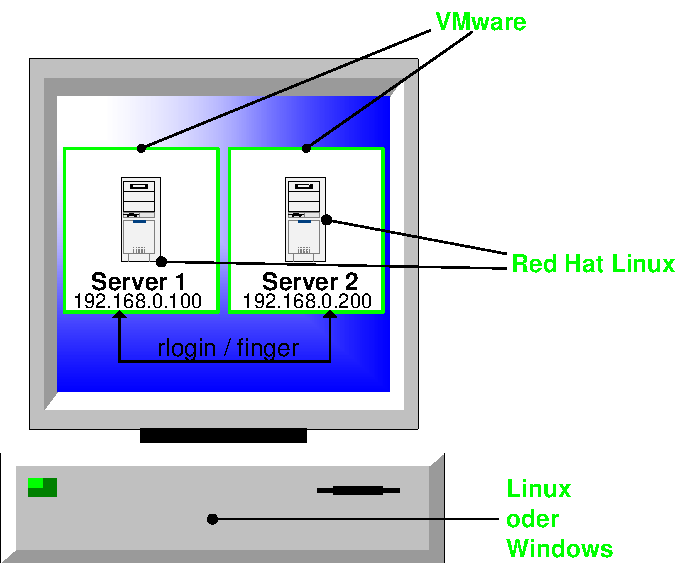
\includegraphics[width=10cm]{./files/inc/pictures/pdf/uebungsuebersicht}
		\caption{\label{pic:uebungsumgebung2}Uebungsumgebung}
	\end{center}
\end{figure}

\section{Entscheid}
\index{Evaluation!Entscheid!�bung}
Die �bungsvariante 1 ist davon abh�ngig, wieviele erfolgreiche Attacken inszeniert werden k�nnen. Solche funktionierenden Attacken f�r ein bestimmtes System zu finden ist sehr aufwendig. Attacken selber zu programmieren �berstieg das zur Verf�gung stehende Zeitbudget bei weitem (siehe Anhang \ref{cha:EvaluationEinerAttacke} auf Seite \pageref{cha:EvaluationEinerAttacke}).
Die �bungsvariante 2 bietet wie Variante 1 die M�glichkeit Techniken des H�rtens anzuwenden. Anstatt Attacken werden nun nicht deaktivierte, sicherheitskritische Dienste zum Aufzeigen von Systemschw�chen genutzt. 
 



	\chapter{Evaluation einer Attacke\index{Evaluation!Exploit}\index{Exploit!Evaluation}}
\label{cha:EvaluationEinerAttacke}
Um den Vorteil eines mit PitBull\index{Pitbull} gesicherten Servers am Besten zeigen zu k�nnen, ist eine der m�chtigsten Attacken auf einen Server n�tig. Dazu geh�rt das direkte erlangen von Root-Rechten �ber einen Remote Zugang. Dies bedeutet, dass von einem, �ber das Netzwerk erreichbaren Rechner jemand die M�glichkeit erlangt, auf dem angegriffenen System beliebige Befehle auszuf�hren. Einem solchen Angriff entspricht die \emph{Bufferovwerflow Attacke}\index{Bufferoverflow Attacke} (genauer erkl�rt im folgenden Abschnitt \ref{sec:BufferoverflowAttacke}).

Als Erstes werden neue Sicherheitsl�cken auf dem Internet publiziert. Darum wurde f�r die Suche nach Informationen �ber eine solche Attacke vor allem dieses Medium verwendet.
\section{Bufferoverflow Attacke}
\label{sec:BufferoverflowAttacke}
\index{Bufferoverflow Attacke}\index{Stack}
Diese Attacke nutzt Schwachstellen in der Implementation von Programmen aus, denen Parameter oder andere zu verarbeitende Daten �bergeben werden k�nnen. Die Schw�che besteht darin, dass bei der Verarbeitung von �bergebenen Daten, diese Daten in den Hauptspeicher kopiert werden, ohne dass die Gr�sse des daf�r reservierten Speicherbereichs �berpr�ft wird. Wird Beispielsweise als Parameter ein String von einer gewissen L�nge erwartet, doch ein weitaus l�ngerer String �bergeben, wird trotzdem der ganze String in den Speicher geschrieben. Dabei werden andere Daten, die sich ebenfalls im Speicher befinden �berschrieben. Falls sich das Programm in diesem Moment gerade innerhalb einer Subroutine befindet, befindet sich auch die R�cksprungadresse ins Hauptprogramm in diesem Speicherbereich. Ziel der Attacke ist es, diese R�cksprungadresse zu �berschreiben und dabei eine Adresse zu setzten, die in den Bereich des Speichers springt, an dem sich der �bergebenen String befindet. Gelingt dies, wird der Prozessor nach dem durcharbeiten der Subroutine versuchen, den �bergebenen String als Programmcode zu interpretieren. Falls sich in dem String also Maschinencode in der Form von Bin�rwerten (sogenannter \emph{Payload}\index{Payload}) befindet, der �ber einen Methodenaufruf des Betriebssystes eine Shell ausf�hrt, erh�lt der fremde Rechner Zugang zu einer Shell mit den Benutzerrechten des fehlerhaften Programmes.
\section{Programmieren der Attacke}
Um eine solche Attacke durchzuf�hren wurden zuerst Hintergrundinformationen �ber das Prinzip der Attacke gesucht. Als beste Quellen erwiesen sich hierf�r zur Einf�hrung in die Thematik der Artikel "`Das Sicherheitsloch"' aus dem Magazin c't \cite{ctexploit} und zur Vertiefung der Artikel "`Smashing the Stack for Fun"' aus dem Phrack Magazin \cite{phrackexploit}.

Durch das Studium der Prinzipien wurde schnell klar, dass das Erstellen eines eigenen Exploits dieser Art dem Umfang einer ganzen Studienarbeit entsprechen w�rde (Details dazu sind in den oben genannten Quellen zu finden): 
\begin{itemize}
\item Analysieren von Quellcode eines Dienstes auf verletzliche Speicherzugriffe, beziehungsweise Aufrufe von bekannten Funktionen, die beim Speicherzugriff keine Bereichspr�fung der Variable durchf�hren
\item Zusammenstellen des sogenannten Payloads der Attacke (dies sind die notwendigen Befehle in Maschinencode, um einen Betriebssystemaufruf zu t�tigen, der beispielsweise eine Shell �ffnet)
\item Das anzugreifende Programm in einem Debugger ausf�hren, um eine bestimmte Speicheradresse (im Stack) zur Laufzeit des Programmes herauszufinden
\item Ein Programm schreiben, das die Verbindung aufbaut und dem Dienst die n�tigen Daten �bermittelt
\end{itemize}
\section{Entscheid}
\index{Evaluation!Entscheid!Programmieren eines Exploits}
Um eine solche Attacke selber zu programmieren stand nicht gen�gend Zeit zur Verf�gung. Aus diesem Grund wurde entschieden, auf dem Internet nach bereits vorhandenen Attacken f�r den Standard Server der �bungsinstallation aus Abschnitt \ref{subsec:VirtuelleServer} zu suchen.
\section{Suche nach einem Exploit}
Zuerst wird der Verlauf der Suche beschrieben und die genutzten Informationsquellen genannt. Anschliessend werden weitere Anregungen f�r eine Suche genannt.

Bei der Suche nach einem Exploit wurden verschiedene Strategien verfolgt. Zuerst wurde eine sehr eingegrenzte Suche durchgef�hrt, anschliessend wurden die Kriterien des Exploits immmer mehr gelockert. Grob k�nnte die Suche und in folgende Phasen eingeteilt werden:
\begin{enumerate}
	\item Suche nach Exploits f�r die installierten Softwarepakete des aufgesetzten Standard Servers mit Red Hat 7.3
	\item Suche nach Exploits f�r �ltere Versionen der installierten Softwarepakete
	\item Suche nach Exploits einer beliebigen lauff�higen Software unter Red Hat 7.3
\end{enumerate}
Im Folgenden sind die Ergebnisse der einzelnen Phasen zusammengefasst. Eine Auswahl der gefunden Scripte sind auf der beigelegten CD zu finden (\ref{cha:BeiliegendeCds} auf Seite \pageref{cha:BeiliegendeCds}).:
\begin{enumerate}
	\item Es wurden zwei Skripte f�r den \emph{Apache Server} gefunden, die aber nicht die erwarteten Reaktionen zeigten, bzw. nicht funktionierten.
	\item F�r eine �ltere Version des \emph{Apache Servers} wurden verschiedene Scripte f�r die gleiche Schwachstelle gefunden. Die Apacheversion auf dem Server wurde durch eine �ltere Version ersetzt. Dies galt auch f�r alle abh�ngigen Pakete. Dennoch erwies sich kein Script als tauglich.
	\item Es wurde auf verschiedenen Webseiten auf eine Schwachstelle einer �lteren Version des FTP-Serverprogrammes \emph{ProFTP} hingewiesen. Nach der Installation des Programmes wurde ein FTP-Exploit-Script ausgef�hrt, jedoch ohne Erfolg.
\end{enumerate}
\section{Informationskan�le}\index{Exploit!Quellen}
Eine Auswahl der besuchten Internetseiten, die nach Informationen durchsucht wurden:
\begin{description}
	\item [online.securityfocus.com]Sehr Umfangreiche Datenbank bez�glich Computer Sicherheit
	\item [packetstormsecurity.nl]Sehr umfangreiche Datenbank mit diversen Exploit-Be\-schreibungen inklusive Quellcode. Das Motto der Organisation \emph{Packet Storm} ist "`Know your enemy"'.
	\item [www.phrack.org]Das Hacker und Phreak Magazin �berhaupt. Es bietetet neue kreative Ideen f�r Hacking Ans�tze.
	\item [www.cultdeadcow.com]Seite einer Hackergruppe. Sie bieten ein paar wenige Tools und News an.
	\item [www.atstake.com]Eine Netzwerksicherheit-Beratungs Firma in Amerika. Sie bietet verschiedene ausgekl�gelte Netzwerksicherheit-Tools an. Unter anderem auch solche, die Applikationen auf potentielle Bufferoverflow-Fehler pr�fen.
\end{description}
Alternativ befragten wir Mitglieder der LUGS (Linux User Group) ein Linux-Verein an der Hochschule Rapperswil, die uns einzelne der oben genannten Webseiten verwiesen.
\section{Ungenutzte Informationskan�le}\index{Exploit!Informationsquellen}
Der Internet Relay Chat (IRC)\index{IRC} bietet eine intensiv genutzte Plattform zum Infor\-ma\-ti\-ons- und Pro\-grammaustausch. Unter anderen auch zu Themen die sich in Grauzonen der Legalit�t befinden. Um diese Quellen allerdings gezielt und effizient nutzen zu k�nnen, muss man sich w�hrend einer gewissen Zeit (Sch�tzungsweise ein bis zwei Monaten) in den verschiedenen Chatr�umen und auf den verschiedenen Servern "`bewegen"', beziehungsweise Kontakte kn�pfen und Informationen sammeln. �ber diese Vorarbeit erh�lt man Wissen �ber nicht offizielle und versteckte Chatr�ume, wie auch Aufenthalt und Commandos f�r sogenannte Bots\footnote{Bots sind Dienste, die sich wie reale Chatpersonen in Chatr�umen aufhalten und auf eingegebenen Text reagieren (Zum Beispiel Scripte ausf�hren oder Dateitransfers einleiten).}. Die auf IRC gehandelten Informationen sind oft brisanter, als die auf Webseiten publizierten, da Benutzer miteinander kommunizieren k�nnen, ohne dass sie ihre IP-Adressen preisgeben m�ssen\footnote{IRC Server versenden die Nachrichten an die bei ihnen angemeldeten Clients.}.

Die Suche nach Informationen in verschiedenen Newsgroups w�re ebenfalls eine Alternative, ben�tigt aber Erfahrungen bez�glich der Qualit�t der einzelnen Gruppen.

Das Anmelden bei Mailinglisten zu den entpsrechenden Themen k�nnte sich auch als hilfreich erweisen bei der Suche nach Exploits, kann sich aber durch das Verarbeiten von ganzen Mailfluten als sehr zeitaufwendig entpuppen.
\section{Fazit der Exploit-Suche}\index{Evaluation!Exploit!Fazit}
Die Suche nach einem Exploit, der f�r eine spezifische Systemkonfiguration geschrieben wurde, ist sehr aufwendig. Es gibt verschiedene Variablen der Systemkonfiguration, die mit dem Exploit �bereinstimmen m�ssen. Dazu geh�ren die Version des Betriebssystems (oft auch die Version des Kernels) und die Version des anzugreifenden Dienstes. Beim \emph{Apache Server} sind auch die Versionen der installierten Module relevant. Bei einem Angriff auf den \emph{Apache Server}\index{Apache Server} gibt dies bereits mindestens vier Variablen die mit dem Exploit �bereinstimmen m�ssen. Falls nur eine Handvoll Exploits f�r den Apache gefunden werden, ist es unwahrscheinlich, dass einer der Exploits funktioniert.
Zudem ist der Sourcecode von gefundenen Exploits meistens von sehr schlechter Qualit�t. Unter schlechter Qualit�t wird folgendes verstanden:\index{Exploit!Qualit�t}
\begin{itemize}
\item Schlecht bis gar nicht kommentiert (geschweige den Dokumentiert) 
\item kaum aussagekr�ftige Fehlermeldungen oder gar keine Fehlermeldungen implementiert
\item fehlerhafter Code (Typendeklaration falsch, Methodenaufrufe mit falscher Anzahl Argumenten, usw.)
\item Variablen- und Methodennamen nicht in Englisch (gefunden wurden Scripte in Spanisch)
\end{itemize}
Dies hat verschiedene Gr�nde: Der Code war nicht f�r die Weitergabe gedacht, nur f�r den Eigenbedarfentwickelt und/oder Codeteile wurden zusammenkopiert aus "`in the wild"' entdeckten, b�sartigen Programmen (z.B. aus einem Wurm).
Um ein gefundenes Script benutzen zu k�nnen, sind oft folgende Massnahmen erforderlich:
\begin{itemize}
	\item Fehler finden und korrigieren
	\item Programmlogik genau analysieren und gegebenfalls anpassen
	\item in Machinencode integrierter Payload (Siehe Abschnitt \ref{sec:BufferoverflowAttacke} "`Bufferoverlow Attacke"') f�r das anzugreifende System selber schreiben, kompilieren und in das Script einf�gen, damit die Betriebssystemversion sicher stimmt.
\end{itemize}
Es folgt ein Auszug aus der Datei \verb~apache-scalp.c~ mit einem Kommentar der Entwickler zur Illustration des Aufwandes die mit einem funktionierenden Exploit-Script verbunden sind.
\begin{verbatim}
 * The "experts" have already concurred that this bug...
 *      -       Can not be exploited on 32-bit *nix variants
 *      -       Is only exploitable on win32 platforms
 *      -       Is only exploitable on certain 64-bit systems
 *
 * However, contrary to what ISS would have you believe, we have
 * successfully exploited this hole on the following operating systems:
 *
 *      Sun Solaris 6-8 (sparc/x86)
 *      FreeBSD 4.3-4.5 (x86)
 *      OpenBSD 2.6-3.1 (x86)
 *      Linux (GNU) 2.4 (x86)
 *
 * Don't get discouraged too quickly in your own research. It took us
 * close to two months to be able to exploit each of the above operating
 * systems. There is a peculiarity to be found for each operating system 
 * that makes the exploitation possible.
\end{verbatim}
Dieser Kommentar sagt nicht nur aus, dass es Monate dauern kann bis ein spezieller Exploit funktioniert, sondern sich Sicherheitsexperten oft selber nicht einig sind, f�r welche Systeme ein Exploit jetzt funktioniert oder nicht.
Es scheint schwieriger zu sein f�r ein konkretes System einen funktionierenden Exploit zu finden, als mit einem Exploit-Script auf dem ganzen Internet ein angreifbares System.
\section{Entscheid}\index{Evaluation!Entscheid!Attacken}
Die Exploit-Suche zeigte sich trotz verschiedenen Ans�tzen und Nachforschungen ohne Erfolg. Da ein solcher Exploit die Basis f�r die �bung mit PitBull darstellte, wurde der �bungsablauf �berarbeit. Der neue �bungsablauf war nun, die Hardening Theorie anzuwenden und nicht mehr drei verschieden Server zu vergleichen (Siehe \ref{sec:UebungVariante2} auf Seite \pageref{sec:UebungVariante2}). 

	\chapter{Hardware Evaluation\index{Evaluation!Hardware}}
\label{cha:HardwareEvaluation}
Im Verlauf der Arbeit standen nacheinander zwei verschiedene Server mit unterschiedlich leistungsf�higen Komponenten f�r Testzwecke zur Verf�gung (im Folgenden mit "`Alpha Lab"' und "`Beta Lab"' bezeichnet). Auf beiden Rechnern wurde Red Hat 7.3 und VMware Workstation Version 3.2 installiert. Im Folgenden werden die Hardwarekonfigurationen der beiden Systeme und das Verhalten der Systeme w�hrend dem Einrichten und den ersten Funktionstests geschildert, um einen Eindruck �ber die Anforderungen zu vermitteln.
%----------
\section{Alpha Lab}
\label{sec:AlphaLab}
Das zur Verf�gung stehende Hostsystem hat folgende Hardwaredaten:
\begin{itemize}
\item 3.2 GB Festplatte
\item Hauptspeicher 128 MB
\item Intel Pentium II, 266 MHz
\item ATI Mach64, 4 MB RAM
\item Microsoft Maus (PS/2), zwei Kn�pfe
\item SVGA f�higer Bildschirm
\item Standard 105 Tasten Keyboard
\end{itemize}
Es konnten maximal zwei virtuelle Systeme gleichzeitig gestartet werden. Pro Systemen stand maximal 32 MB Hauptspeicher zur Verf�gung. Die Anzahl parallel aufgesetzter Systeme wurde auch durch die zur Verf�gung stehende Festplattenkapazit�t stark eingeschr�nkt. Pro Server sollte mindestens 1 GB zur Verf�gung stehen. Davon wird 1 GB bereits vom Hostsystem selbst verwendet. Die Systemreaktionen der virtuellen Systeme waren sehr tr�ge. Die Konfigurationen aus den Konsolen der simulierten Server waren noch gut m�glich. Der Bildaufbau dauerte teilweise ein bis zwei Sekunden. Bei Webzugriffen von einem beliebigen System im Uebungsnetz war nicht ersichtlich, dass es sich nur um einen simulierten Server handelte. Um zwei Webserver, ohne zus�tzliche Dienste f�r eine �bung zu simulieren, w�rden diese Hardwarevoraussetzungen reichen. Das System w�re aber sehr verletzlich gegn�ber einer \emph{Denial of Service Attacke}.
%------------------
\section{Beta Lab}
\label{sec:BetaLab}
Das zur Verf�gung stehende Hostsystem hat folgende Hardwaredaten:
\begin{itemize}
\item 6.4 GB Festplatte
\item Hauptspeicher 512 MB SDRAM
\item Intel Pentium III, 550 MHz
\item ATI Mach64, 16 MB RAM
\item Microsoft Maus (PS/2), zwei Kn�pfe
\item SVGA f�higer Bildschirm
\item Standard 105 Tasten Keyboard
\end{itemize}
Das starten von drei virtuellen Systemen gleichzeitig stellt kein Problem dar. Jedem virtuellen System stehen 128 MB Hauptspeicher zur Verf�gung. Das Arbeiten mit den virtuellen Systemen war ohne gr�ssere, bemerkbare Geschwindigekitseinbussen m�glich.
%------------------
\section{Erkenntnis}
Die Systemvoraussetzungen des Beta Labs waren gegn�ber dem Alpha Lab wesentlich besser. Die Gr�sse der Harddisk reicht zwar aus, l�sst aber f�r die Serverinstallationen nicht allzuviel Spielraum f�r das Installieren von zus�tzlichen Paketen. Es stehen pro System (dem Host System inklusive) 1.6 GB Plattenspeicher zur Verf�gung. Um m�glichen Speicherplatzproblemen vorzubeugen, sollte das Host System mindestens 8 GB Festplattenspeicher besitzen, damit den drei virtuellen Systemen je 2 GB zur Verf�gung stehen. Ansonsten gen�gen die Hardwarevoraussetzungen des Beta Labs den �bungsanforderungen.




	\chapter{Beiliegende CDs\index{CD-Beilage}}
\label{cha:BeiliegendeCds}
Dem Bericht liegen zwei CDs bei. Auf einer CD befindet sich der Bericht, Skripte und Informationen bez�glich dem Projekt, auf der anderen befinden sich die in VMware ausf�hrbaren konfigurierten Server 1 und 2. Dieser Anhang beschreibt den Inhalt der beigelegten CDs.
%----------
\section{CD 1}
\label{sec:Cd1}
\begin{itemize}
\item Bericht in \LaTeX\
\item Bericht im PDF-Format
\item Diagramme aus dem Bericht
\item Exploitcode Beispiele
\item Webseite des Projekts (inkl. Zeitauswertung und Projektplan)
\item VMware Desktop 3.2 f�r Linux (inkl. Lizenz)
\item VMware Desktop 3.2 f�r Windows (ohne Lizenz)
\end{itemize}
%----------
\section{CD 2}
\label{sec:Cd2}
\begin{itemize}
\item VMware Dateien des Server 1
\item VMware Dateien des Server 2
\end{itemize}

	\chapter{Projektmanagement Dokumente}
\section{Zeitauswertung}
Dieser Auszug aus der Datenbank zeigt die Arbeitszeiten geordnet nach Person und Bereich.
\begin{verbatim}
Michael Egli                                             162.00
    Dokumentation       92.00    	
    Einarbeiten         32.00 
    IT Arbeitsumgebung  15.00 
    IT Projektbezogen    1.00 
    Meeting             11.25 
    Projektmanagement   10.75 

Ren� Herrmann                                            155.75
    Dokumentation       63.50 
    Einarbeiten         26.25 
    IT Arbeitsumgebung  18.50 
    IT Projektbezogen   24.75 
    Meeting             10.25 
    Projektmanagement   12.50       
                                 Projekt Total:          317.75 
\end{verbatim}
\section{Projektplan}
Der Projektplan befindet sich auf der folgenden Seite.



	%Bitte beim eintragen alphabetisch ordnen
\chapter{Glossar}
\label{cha:Glossar}

\begin{description}
\item[\Large{A}]
\item[ARP] Address Resolution Protocol. Das Protokoll verbindet die IP-Adresse mit der physikalischen MAC-Adresse der jeweiligen Ethernet-Karte.
\item[Authentifizierung] Bezeugen der Echtheit
\item[Authentisierung] Beglaubigung, Rechtsg�ltigmachung

\item[\Large{D}]
\item[Dienst] Ein Programm, dass Funktionen oder Ressourcen zur Verf�gung stellt (Beispielsweise \textit{sshd}).

\item[\Large{H}]
\item[H�rten eines Systems] Vorgehen, um ein System sicherer zu machen.
\item[Host System] System auf welchem VMware installiert ist.

\item[\Large{M}]
\item[MAC] Media Access Control. Dieser Layer bietet die M�glichkeit des individuellen Zugriffs bez�glich der verwendeten Netzarchitektur.

\item[\Large{N}]
\item[Non-Repudiation] Eindeutigkeit des Ursprungs.

\item[\Large{O}]
\item[OS Hardening] Prozess um die Sicherheit eines IT-Systems zu erh�hen.

\item[\Large{P}]
\item[PAM] Pluggable Authentication Module. PAM dient der einheitlichen Authentifizierung der Benutzer durch verschieden Programme.
\item[partitionieren] Die Festplatte in verschiedene Bereiche aufteilen, die untereinander unabh�ngig sind.

\item[\Large{V}]
\item[Virtuelles System] Ein innerhalb von VMware installiertes System, das einen kompletten Rechner simuliert. Die Hardwarekonfiguration des Rechners sind simulierte VMware Komponenten.
\end{description}

	\bibliography{./files/inc/references}
	\label{bibliography}
	\printindex
\end{appendix}

\end{document}
